\documentclass[a4paper, twoside, 12pt]{book}
\usepackage{latexsym}
\usepackage[MeX]{polski}
\usepackage[utf8]{inputenc}
\usepackage{graphicx}
\usepackage{listings}
\usepackage{amsmath}
\usepackage{float}
\usepackage{hyperref}
\usepackage{listings}
\usepackage{fancyhdr}
\usepackage{gensymb}
\usepackage{subfig}
\usepackage{url}
\usepackage[font=it, justification=centering]{caption}
\usepackage{setspace} % ustawienie interlinii
\usepackage{listings}
\usepackage{array}
\usepackage{pdfpages}
\usepackage{ragged2e}
\usepackage{enumitem} % formatowanie marginesów itemize

% numeracja
\pagestyle{fancy}

\raggedbottom
%zmiana stylu z kontynuacja numerowania
\newcounter{savepage}
\newcommand{\setpagenumberingtype}[1]{%
	\setcounter{savepage}{\arabic{page}}%
	\pagenumbering{#1} %
	\setcounter{page}{\thesavepage}%
}

\fancyhead{} % clear all header fields
\renewcommand{\chaptermark}[1]{\markboth{\chaptername\ \thechapter.\ #1}
{}}
\renewcommand{\sectionmark}[1]{\markright{\thesection.\ #1}} 

%\fancyhead[RE]{\bfseries\nouppercase{\leftmark}\sectionmark}      % Chapter in the right on even pages
%\fancyhead[LO]{\bfseries\nouppercase{\rightmark}\chaptermark}     % Section in the left on odd pages
\fancyfoot{} % clear all footer fields
%\renewcommand{\headrulewidth}{0.4pt}
\fancyfoot[LE, RO]{\bfseries \thepage} % except the center
\fancyheadoffset[]{0.4pt}

\renewcommand{\headrulewidth}{0pt}

\fancypagestyle{empty}{%
\fancyhf{} % clear all header and footer fields
\fancyfoot[LE, RO]{\bfseries \thepage} % except the center
}

\fancypagestyle{plain}{%
\fancyhf{} % clear all header and footer fields
%\fancyhead[RE]{\bfseries\nouppercase{\leftmark}}      % Chapter in the right on even pages
\fancyfoot[LE, RO]{\bfseries \thepage} % except the center
%\renewcommand{\headrulewidth}{0pt} %
\renewcommand{\footrulewidth}{0pt}
}

\fancyfoot[LE, RO]{\bfseries \thepage} % except the center


\usepackage[a4paper, left=2.5cm, right=2.5cm, top=3.7cm, bottom=2.5cm, headsep=0.9cm, headheight=16pt]{geometry}
\frenchspacing
\linespread{1.3}
\usepackage{hyperref} % musi być na końcu
\hypersetup{pdfborder={0 0 0 0}}

\newcolumntype{P}[1]{>{\centering\arraybackslash}p{#1}}

\begin{document}
	\setpagenumberingtype{gobble} % Remove page numbers (and reset to 1)

% ŻYCIORYS (z drugiej strony)
\mbox{}
\thispagestyle{empty}
\newpage
% TODO skan podpisanego życiorysu
% 
\includepdf[pages={1}]{attach/cv.pdf}
\begin{figure}[ht]
\begin{doublespacing}
	\begin{minipage}[b]{0.4\linewidth}
		
\includegraphics[width=4cm]{img/cv/me}
	\end{minipage}
	\begin{minipage}[b]{0.5\linewidth}
		Kierunek:  Automatyka i Robotyka \\
		Specjalność:  Informatyka Przemysłowa \\
		Data urodzenia:  21.03.1993 r. \\
		Data rozpoczęcia studiów:  23.02.2016 r. \\
	\end{minipage}
	
	\hspace{2cm}
	
	\begin{center}
		\huge{\textbf{Życiorys}} \\
	\end{center}

Urodziłem się 21. marca 1993 roku w Lublinie. W 2012 roku rozpocząłem studia inżynierskie I stopnia na Wydziale Mechatroniki Politechniki Warszawskiej, na kierunku Automatyka i Robotyka, na specjalności Informatyka Przemysłowa. Ukończyłem je 17 lutego 2016 roku. W tym samym roku rozpocząłem studia II stopnia na tym samym wydziale, na specjalności Informatyka Przemysłowa. \\

	\vspace{2cm}
	% podpis
	\begin{flushright}
				.............................................. \\
	\end{flushright}
\end{doublespacing}
\end{figure}



\clearpage

\setcounter{page}{1} % życiorys nienumerowany
\newgeometry{tmargin=3cm, bmargin=3cm, lmargin=2cm, rmargin=2cm}

% STRONA TYTUŁOWA
\newgeometry{tmargin=3cm, bmargin=3cm, lmargin=2cm, rmargin=2cm}

\thispagestyle {empty}

\begin{center}
	%logo uczelni
	
\includegraphics[scale=0.4]{img/pw}
	
	\vspace{0.5cm}
	
	{\fontsize{20}{20}\selectfont POLITECHNIKA WARSZAWSKA}
	
	\vspace{1.0cm}
	
	\textbf{{\fontsize{14}{14}\selectfont Wydział Mechatroniki}}
	
	\vspace{1.5cm}
	
	\textbf{{\fontsize{14}{14}\selectfont Praca magisterska}}

	\vspace{2.0cm}
	
	{\fontsize{14}{14}\selectfont Ireneusz Szulc}
	
	\vspace{1cm}
	
	{\fontsize{28}{28}\selectfont Planowanie bezkolizyjnych tras dla zespołu robotów mobilnych}
	
	\vspace{1cm}
	\begin{flushright}
		{\fontsize{14}{14}\selectfont Opiekun pracy: \\ 
		prof. nzw. dr hab. Barbara Siemiątkowska
		}
	
		\vspace{1cm}
		
		\vspace{3cm}
		% {\fontsize{14}{14}\selectfont Konsultant pracy: \\ 
		% mgr inż. }
		
	\end{flushright}
	
	\vspace{1cm}
	
	{\fontsize{12}{12}\selectfont Warszawa, 2018}
	
	%\cleardoublepage %nie działa
	
	%\clearpage\mbox{}\clearpage
\end{center}
% TODO karta tematu wygenerowana z USOSa
% \includepdf[pages={1}]{attach/title-page.pdf}
\clearpage{\pagestyle{empty}\cleardoublepage}
\cleardoublepage

% KARTA TEMATU
\phantomsection
% TODO skan podpisanej karty
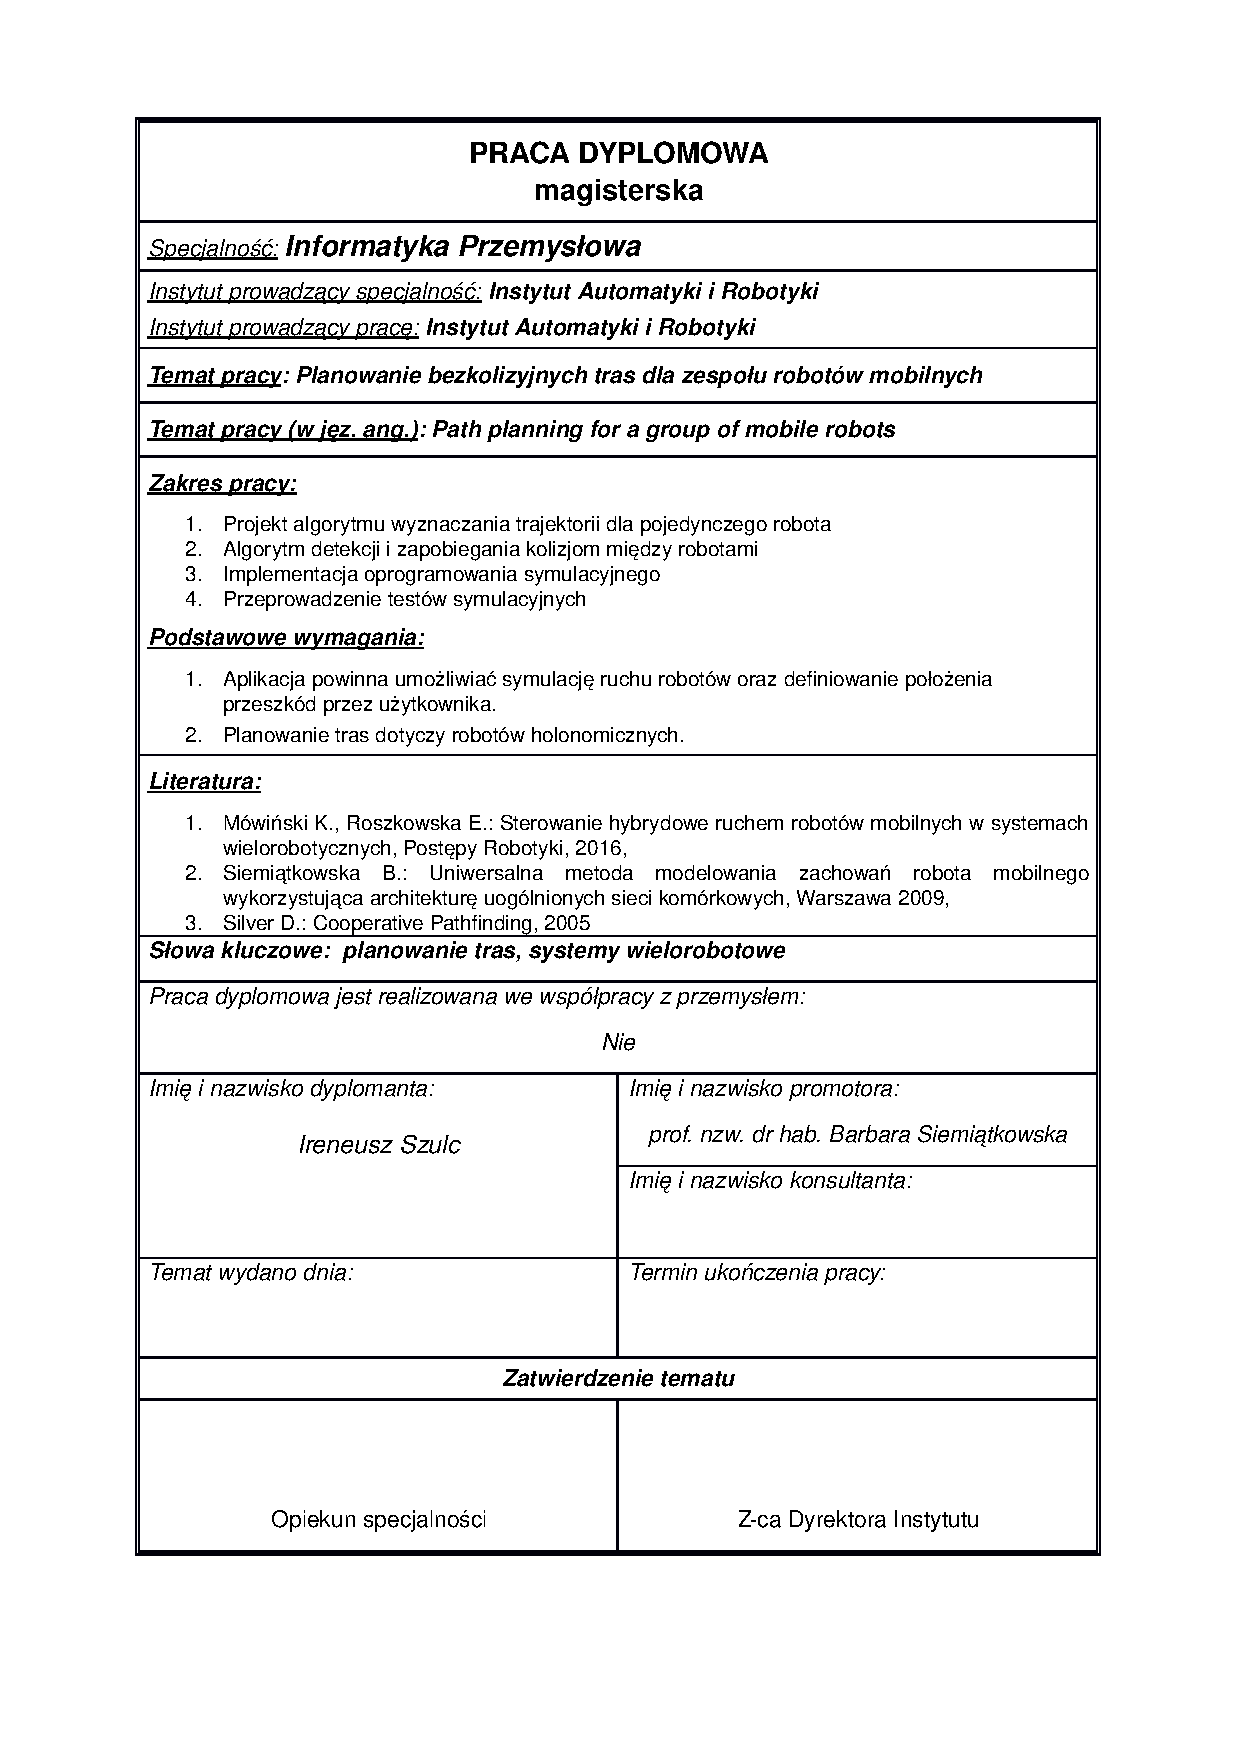
\includepdf[pages={1}]{attach/karta-tematu.pdf}
\cleardoublepage

% STRESZCZENIA
\noindent {\Large\textbf{Streszczenie}}\\

\noindent {\Large\textbf{Planowanie bezkolizyjnych tras dla zespołu robotów mobilnych}}\\

% interlinia 0
\begin{singlespacing}

Przedmiotem niniejszej pracy jest przegląd, implementacja i wykonanie testów wybranych metod planowania bezkolizyjnych tras dla systemów wielorobotowych.
W ramach pracy zostały opracowane własne metody wyznaczania dróg dla wielu robotów mobilnych na dwuwymiarowych mapach.
Metody te znajdują zastosowanie w środowiskach z dużą liczbą przeszkód i wąskimi gardłami, gdzie często występuje problem zakleszczania się robotów.

% wstęp teoretyczny - przegląd metod
W pierwszych rozdziałach dokonano przeglądu i analizy najczęściej wykorzystywanych podejść do kooperacyjnego planowania tras.
Wskazano również na podobieństwo występowania podobnego zagadnienia w grach komputerowych.

% algorytmy
W kolejnej części omówiono algorytmy opracowane na potrzeby oprogramowania symulacyjnego.
Efektem pracy jest m.in. własna implementacja algorytmu {\it Windowed Hierarchical Cooperative A*} rozszerzonego o dodatkowe procedury dynamicznego przydziału priorytetów oraz zmiennego okna czasowego.

% oprogramowanie symulacyjne
W ramach pracy wykonano oprogramowanie pozwalające na symulację oraz wizualizację metod planowania tras w systemach wielorobotowych.
Opracowana aplikacja desktopowa realizuje założone funkcjonalności.
Użytkownik ma możliwość dowolnego definiowania środowiska a wizualizacja ruchu robotów mobilnych odbywa się w czasie rzeczywistym.
W jednym z rozdziałów zostały omówione techniczne rozwiązania wykorzystane podczas tworzenia aplikacji.

% testy
Stworzone oprogramowanie symulacyjne posłużyło również do przeprowadzenia testów skuteczności algorytmów planowania tras.
W kolejnej części przedstawiono wyniki automatycznie przeprowadzonych testów zaimplementowanych metod planowania.
Wykonanie licznych eksperymentów pozwoliło stwierdzić, że opracowana własna metoda uzyskała największą skuteczność w wyznaczaniu bezkolizyjnych tras i prowadzeniu agentów do ich celów w porównaniu do pozostałych wariantów.
Na potrzeby wszystkich testów efektywności oraz wydajności badanych metod przeprowadzono łącznie $76\ 800$ automatycznie zarządzanych symulacji ruchu robotów.
Testy te były przeprowadzane w losowo wygenerowanych środowiskach, w różnych warunkach.
W celu generalizacji uzyskanych wyników posłużono się statystyką.


Zauważalny brak ogólnie dostępnych, wydajnych i efektywnych algorytmów kooperacyjnego planowania dróg świadczy o potrzebie rozwoju i rozpowszechnienia metod tego typu, co także było celem tej pracy i zostało zrealizowane poprzez opublikowanie kodów źródłowych opracowanej aplikacji na portalu dla projektów typu {\it open-source}.

Na podstawie obserwacji zachowań robotów sterowanych przez opracowaną metodę planowania tras można niejednokrotnie stwierdzić, że roboty te potrafią wykazywać się "inteligentną" koordynacją ruchu.
Przystosowując się do zmiennych warunków, roboty potrafią niekiedy podejmować akcje, które z pozoru nie byłyby korzystne dla indywidualnego agenta (np. oddalają go od celu), jednak pozwalają one osiągnąć wspólny cel dzięki koooperacji.

\flushbottom
\textbf{\\Słowa kluczowe: }planowanie tras, systemy wielorobotowe
\end{singlespacing}

\cleardoublepage
\noindent {\Large\textbf{Abstract}}\\

\noindent {\Large\textbf{Path planning for a group of mobile robots}}\\

% interlinia 0
\begin{singlespacing}

$TODO$ przetłumaczyć

\flushbottom
\textbf{\\Key words: }cooperative path-planning, multi-agent systems
\end{singlespacing}

\cleardoublepage

% OŚWIADCZENIE AUTORA PRACY

\includepdf[pages={1}]{attach/oswiadczenie_autora_pracy.pdf}
\cleardoublepage

% SPIS TREŚCI
\phantomsection
\addcontentsline{toc}{chapter}{Spis treści}
\tableofcontents
\clearpage

\raggedbottom
\setpagenumberingtype{arabic} % kontynuowanie numerowania w stylu arabskim
% ROZDZIAŁY

\chapter{Wstęp}
\label{ch:wstep}

\section{Cel i zakres pracy}
Przedmiotem niniejszej pracy jest przegląd metod wykorzystywanych do planowania bezkolizyjnych tras dla wielu robotów mobilnych.
Stanowi to również wstęp teoretyczny do zaprojektowania algorytmu i implementacji oprogramowania pozwalającego na symulację działania skutecznego planowania tras dla systemu wielorobotowego.

Praca skupia się na przypadkach, w których mamy do czynienia ze środowiskiem z dużą liczbą przeszkód (np. zamknięty budynek z licznymi ciasnymi korytarzami), aby uwypuklić  problem blokowania sią agentów często prowadzący do zakleszczenia. Często okazuje się, że należy wtedy zastosować nieco inne podejścia niż te, które sprawdzają się w przypadku otwartych środowisk, a które zostały opisane np. w pracach \cite{roszkowska}, \cite{siemiatkowska}.
W otwartych środowiskach z małą liczbą przeszkód wystarczające może się okazać np. proste replanowanie wykorzystujące algorytm D* (por. \ref{ch:dstar}) lub LRA* (por. \ref{ch:lra}).

W niniejszej pracy starano się znaleźć metody rozwiązujące zagadnienie, w którym znane są:
\vspace{-1em}
\begin{itemize}[noitemsep]
	\item pełna informacja o mapie otoczenia (położenie statycznych przeszkód),
	\item aktualne położenie i położenie celu każdego z robotów.
\end{itemize}
Szukany jest natomiast przebieg tras do punktów docelowych dla agentów. Zadaniem algorytmu będzie wyznaczenie możliwie najkrótszej bezkolizyjnej trasy dla wszystkich robotów. Należy jednak zaznaczyć, że priorytetem jest dotarcie każdego z robotów do celu bez kolizji z innymi robotami. Drugorzędne zaś jest, aby wyznaczone drogi były możliwie jak najkrótsze.

\clearpage
\subsection{Założenia}
\label{ch:zalozenia}
Założenia i ograniczenia rozważanego problemu:
\begin{enumerate}
	\item Każdy z robotów ma wyznaczony inny punkt docelowy, do którego zmierza.
	\item Planowanie tras dotyczy mobilnych robotów holonomicznych.
	\item Czas trwania zmiany kierunku robota jest pomijalnie mały.
	\item Srodowisko, w którym poruszają się roboty, jest dwuwymiarową przestrzenią zawierającą dużą liczbę przeszkód oraz wąskie korytarze (por. rys. \ref{fig:img_robopath_sample-maze}).
	\item Roboty "wiedzą" o sobie i mogą komunikować się ze sobą podczas planowania tras.
	\item Każdy robot zajmuje w przestrzeni jedno pole. Na jednym polu może znajdować się maksymalnie jeden robot (por. rys. \ref{fig:img_robopath_sample-maze}).
	\item Planowanie tras powinno odbywać się w czasie rzeczywistym.
\end{enumerate}

\begin{figure}[H]
	\centering
	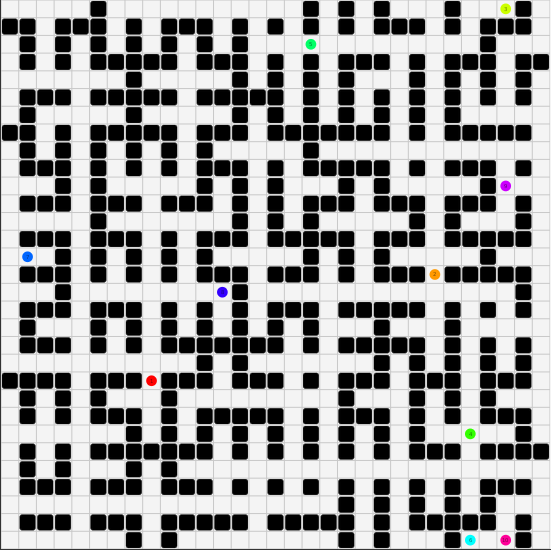
\includegraphics[width=8cm]{img/robopath/sample-maze}
	\caption{Przykładowe środowisko z dużą liczbą przeszkód i rozmieszczonymi robotami. Źródło: własna implementacja oprogramowania symulacyjnego}
	\label{fig:img_robopath_sample-maze}
\end{figure}


\clearpage
\section{Koordynacja ruchu robotów}
Koordynacja ruchu robotów jest jednym z fundamentalnych problemów w systemach wielorobotowych. \cite{optpriorities}

Kooperacyjne znajdowanie tras (ang. {\it Cooperative Pathfinding}) jest zagadnieniem planowania w układzie wieloagentowym, w którym to agenci mają za zadanie znaleźć bezkolizyjne drogi do swoich, osobnych celów. Planowanie to odbywa się w oparciu o pełną informację o środowisku oraz o trasach pozostałych agentów. \cite{cooppath}

Algorytmy do wyznaczania bezkolizyjnych tras dla wielu agentów (robotów) mogą znaleźć zastosowanie w szpitalach (np. roboty TUG i HOMER do dostarczania sprzętu na wyposażeniu szpitala \cite{tughomer}) oraz magazynach (np. roboty transportowe w magazynach firmy Amazon \ref{fig:image_kiva_amazon}).

\begin{figure}[H]
	\centering
	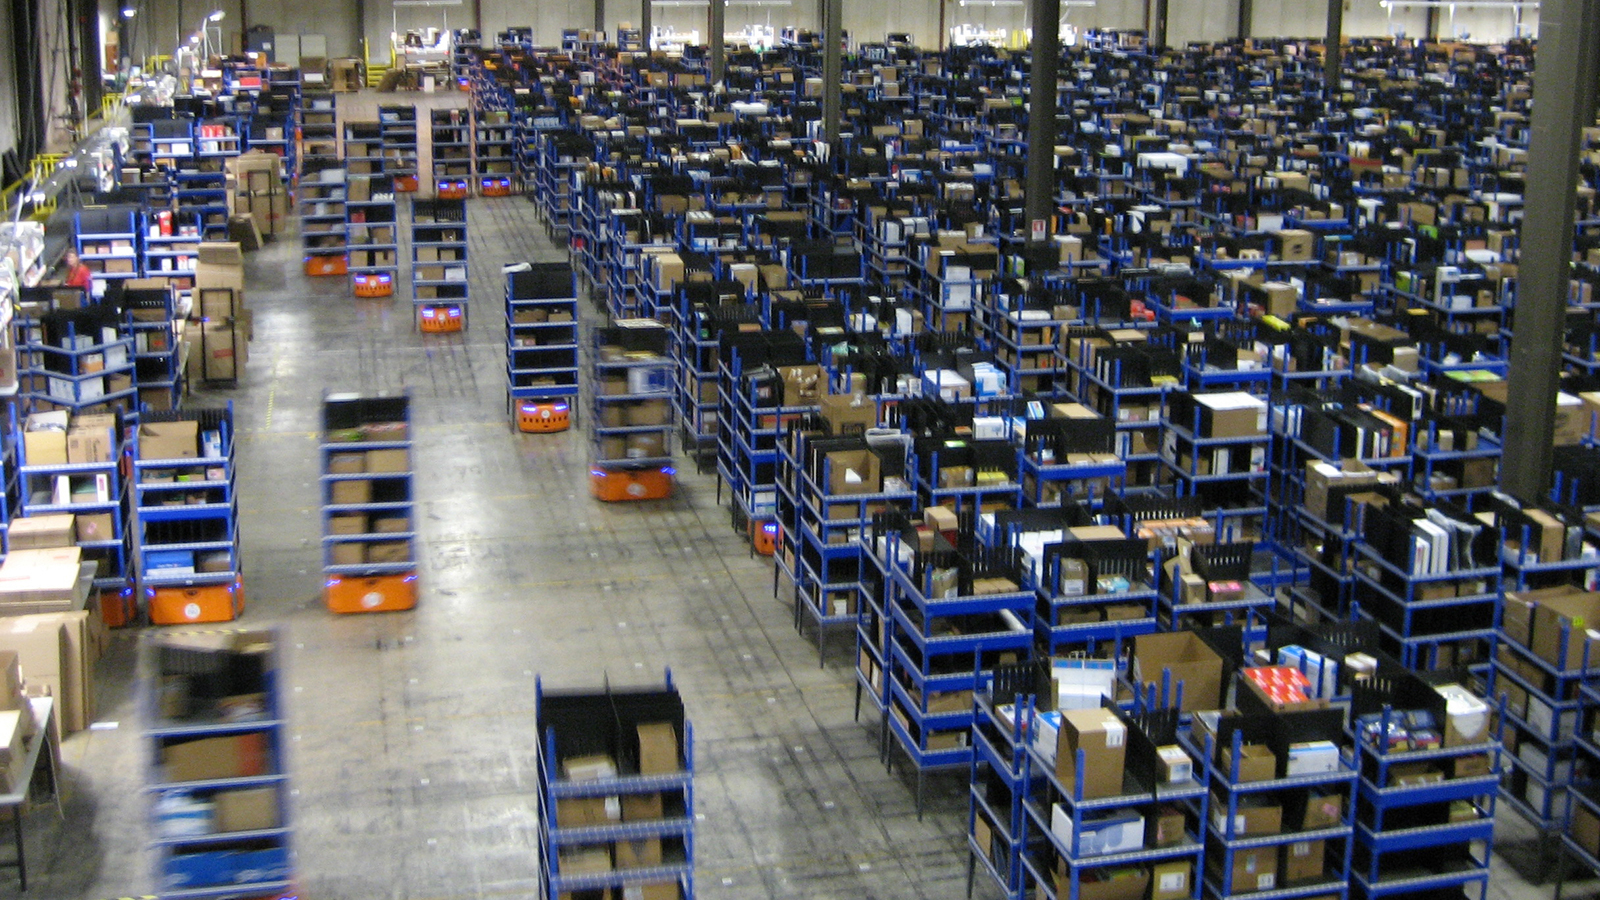
\includegraphics[width=14cm]{img/kiva-amazon}
	\caption{Roboty Kiva pracujące w magazynie firmy Amazon. Źródło: \cite{amazonkiva}}
	\label{fig:image_kiva_amazon}
\end{figure}

\subsection{Podobieństwo do gier RTS}
Problem kooperacyjnego znajdowania tras pojawia się nie tylko w robotyce, ale jest również popularny m.in. w grach komputerowych (strategiach czasu rzeczywistego), gdzie konieczne jest wyznaczanie bezkolizyjnych dróg dla wielu jednostek, unikając wzajemnego blokowania się. Niestety brak wydajnych i skutecznych algorytmów planowania dróg można zauważyć w wielu grach typu RTS (ang. {\it Real-Time Strategy}), gdzie czasami obserwuje się zjawisko zakleszczenia jednostek w wąskich gardłach (np. Age of Empires II, Warcraft III lub nawet we współczesnych produkcjach) \cite{efficient_coop_pathplanning} (por. rys. \ref{fig:img_games_age-deadlock}). Ponadto, zauważalny brak ogólnie dostępnych bibliotek open-source do rozwiązania problemu typu {\it Cooperative Pathfinding} świadczy o potrzebie rozwoju tych metod.

Często algorytmy wykorzystywane w grach typu RTS (ang. {\it Real-Time Strategy}) zajmują się planowaniem bezkolizyjnych dróg dla układu wielu agentów w czasie rzeczywistym (będącego przedmiotem niniejszej pracy), dlatego nic nie stoi na przeszkodzie, aby stosować je zamiennie również do koordynacji ruchu zespołu robotów mobilnych.

\begin{figure}[H]
	\centering
	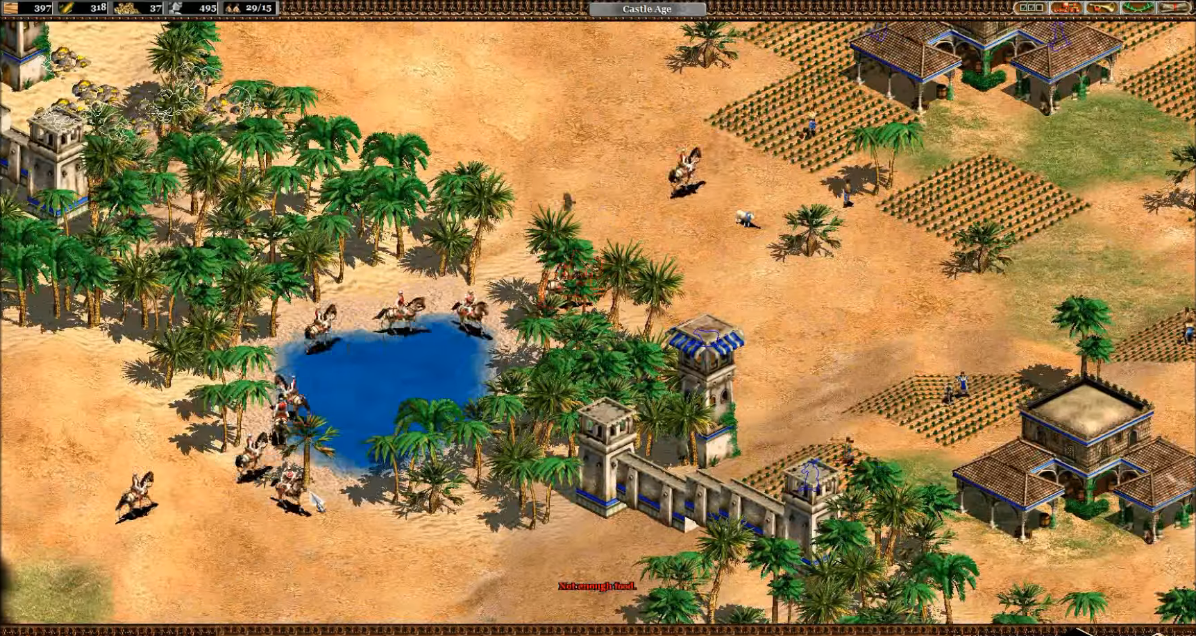
\includegraphics[width=14cm]{img/games/age-deadlock}
	\caption{Popularny problem zakleszczania się jednostek w wąskich gardłach występujący w grach typu RTS. Źródło: gra komputerowa Age of Empires II HD}
	\label{fig:img_games_age-deadlock}
\end{figure}

\section{Podstawowe pojęcia}
\subsubsection{Robot holonomiczny}
Robot holonomiczny to taki robot mobilny, który może zmienić swoją orientację, stojąc w miejscu.

\subsubsection{Przestrzeń konfiguracyjna}
Przestrzeń konfiguracyjna to $N$-wymiarowa przestrzeń będąca zbiorem możliwych stanów danego układu fizycznego.
Wymiar przestrzeni zależy od rodzaju i liczby wyróżnionych parametrów stanu.
W odróżnieniu od przestrzeni roboczej, gdzie robot ma postać bryły, w przestrzeni konfiguracyjnej robot jest reprezentowany jako punkt.

\subsubsection{Zupełność algorytmu (ang. {\it Completeness})}
W kontekście algorytmu przeszukiwania grafu algorytm zupełny to taki, który gwarantuje znalezienie rozwiązania, jeśli takie istnieje.
Warto zaznaczyć, że nie gwarantuje to wcale, że znalezione rozwiązanie będzie rozwiązaniem optymalnym.

% TODO-MGR
% \subsubsection{Metoda hill-climbing}
% Metoda hill-climbing jest rodzajem matematycznej optymalizacji, lokalną metodą przeszukiwania.
% Jest to iteracyjny algorytm, który zaczyna w wybranym rozwiązaniu problemu, następnie próbuje znaleźć lepsze rozwiązanie poprzez przyrostowe zmiany pojedynczych elementów rozwiązania.
% Jeśli przyrostowa zmiana przynosi lepsze rozwiązanie, jest ona wprowadzana do nowego rozwiązania.
% Kroki algorytmu powtarzane są dotąd, aż żadna zmiana nie przynosi już poprawy.


\chapter{Wstęp teoretyczny}
\label{ch:theory}

\section{Podstawowe pojęcia}
\subsubsection{Robot holonomiczny}
Robot holonomiczny to taki robot mobilny, który może zmienić swoją orientację, stojąc w miejscu.

\subsubsection{Przestrzeń konfiguracyjna}
Przestrzeń konfiguracyjna to $N$-wymiarowa przestrzeń będąca zbiorem możliwych stanów danego układu fizycznego.
Wymiar przestrzeni zależy od rodzaju i liczby wyróżnionych parametrów stanu.
W odróżnieniu od przestrzeni roboczej, gdzie robot ma postać bryły, w przestrzeni konfiguracyjnej robot jest reprezentowany jako punkt.

\subsubsection{Zupełność algorytmu (ang. {\it Completeness})}
W kontekście algorytmu przeszukiwania grafu algorytm zupełny to taki, który gwarantuje znalezienie rozwiązania, jeśli takie istnieje.
Warto zaznaczyć, że nie gwarantuje to wcale, że znalezione rozwiązanie będzie rozwiązaniem optymalnym.

% \subsubsection{Metoda hill-climbing}
% Metoda hill-climbing jest rodzajem matematycznej optymalizacji, lokalną metodą przeszukiwania.
% Jest to iteracyjny algorytm, który zaczyna w wybranym rozwiązaniu problemu, następnie próbuje znaleźć lepsze rozwiązanie poprzez przyrostowe zmiany pojedynczych elementów rozwiązania.
% Jeśli przyrostowa zmiana przynosi lepsze rozwiązanie, jest ona wprowadzana do nowego rozwiązania.
% Kroki algorytmu powtarzane są dotąd, aż żadna zmiana nie przynosi już poprawy.

\section{Kooperacyjne planowanie tras}
\label{ch:cooperative_pathfinding}

% \section{Metody planowania tras}
Spośród metod wykorzystywanych do kooperacyjnego planowania tras dla wielu robotów można wyróżnić dwie zasadnicze grupy \cite{latombe}:
\begin{itemize}
	\item {\bf Zcentralizowane} - drogi wyznaczane są dla wszystkich agentów na raz (jednocześnie). Metody tego typu są często trudne do zrealizowania (gdyż do rozwiązania jest złożony problem optymalizacyjny) oraz mają bardzo dużą złożoność obliczeniową ze względu na ogromną przestrzeń przeszukiwania. Struktura organizacyjna jest scentralizowana - decyzje podejmowane są na podstawie centralnego systemu.
	\item {\bf Rozproszone} (ang. {\it decoupled} lub {\it distributed}) - podejście to dekomponuje zadanie na niezależne lub zależne w niewielkim stopniu problemy dla każdego agenta. Dla każdego robota droga wyznaczana jest osobno, w określonej kolejności, następnie rozwiązywane są konflikty (kolizje dróg).
	Zastosowanie metod rozproszonych wiąże się najczęściej z koniecznością przydzielania priorytetów robotom, co stanowi istotny problem, gdyż od ich wyboru może zależeć zupełność algorytmu. Nie należy mylić tej metody z zagadnieniem typu {\it Non-Cooperative Pathfinding}, w którym agenci nie mają wiedzy na temat pozostałych planów i muszą przewidywać przyszłe ruchy pozostałych robotów \cite{cooppath}. W podejściu rozproszonym agenci mają pełną informację na temat stanu pozostałych robotów, lecz wyznaczanie dróg odbywa się w określonej kolejności.
\end{itemize}

W systemach czasu rzeczywistego istotne jest, aby rozwiązanie problemu planowania tras uzyskać w krótkim, deterministycznym czasie, dlatego w tego typu systemach chętniej używane są techniki rozproszone.

\section{Metoda pól potencjałowych}
\label{ch:theory-potential-fields}
Metoda pól potencjałowych (ang. {\it Artificial Potential Field} lub {\it Potential Field Technique}) polega na odwzorowaniu w ruchu robotów zasad oddziaływania między ładunkami elektrycznymi. Roboty i przeszkody reprezentowane są jako ładunki jednoimienne, przez co "odpychają się" siłą odwrotnie proporcjonalną do kwadratu odległości (dzięki temu unikają kolizji między sobą). Natomiast punkt docelowy robota jest odwzorowany jako ładunek o przeciwnym biegunie, przez co robot jest "przyciągany" do celu.
Główną zasadę działania metody przedstawiono na rysunku \ref{fig:image_potentialfield}.

Technika ta jest bardzo prosta i nie wymaga wykonywania złożonych obliczeń (w odróżnieniu do pozostałych metod zcentralizowanych).
Niestety bardzo powszechny jest problem osiągania minimum lokalnego, w którym suma wektorów daje zerową siłę wypadkową. Robot zostaje "uwięziony" w takim minimum lokalnym, przez co nie jest w stanie dotrzeć do wyznaczonego celu. Do omijania tego problemu muszą być stosowane inne dodatkowe metody \cite{potentialfield}.
Metoda pól potencjałowych nie daje gwarancji ani optymalności, ani nawet zupełności.
\begin{figure}
	\centering
	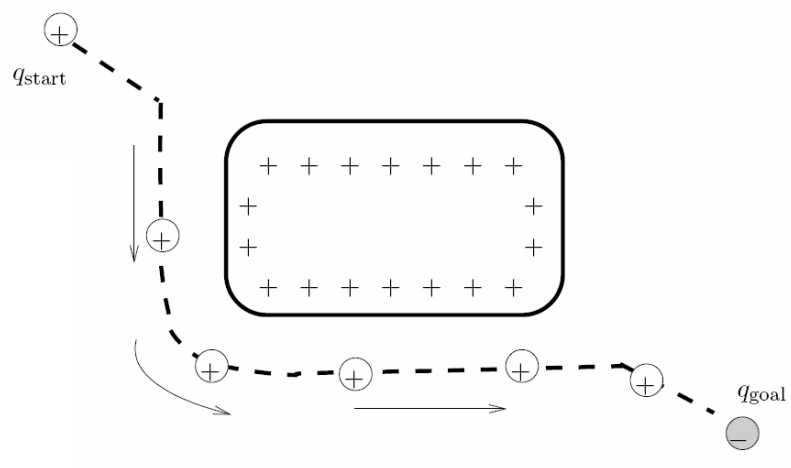
\includegraphics[width=12cm]{img/potential-field}
	\caption{Zasada działania metody pól potencjałowych. Dodatni ładunek $q_{start}$ reprezentuje robota. Przyciągany jest w stronę ujemnego ładunku celu $q_{goal}$, zaś odpychany jest od dodatnio naładowanej przeszkody. Źródło: \cite{howie_potentialfield}}
	\label{fig:image_potentialfield}
\end{figure}

\section{Rozproszone planowanie tras}
Najczęściej stosowanymi podejściami są metody oparte o algorytm A* lub jego pochodne.
W celu wykonywania wydajnych obliczeń w algorytmach przeszukujących grafy, nawet w przypadku ciągłej przestrzeni mapy, stosuje się podział na dyskretną siatkę pól (por. rys. \ref{fig:img_games_warcraft-map-editor}) \cite{hierpathfindinginrts}.

\begin{figure}[H]
	\centering
	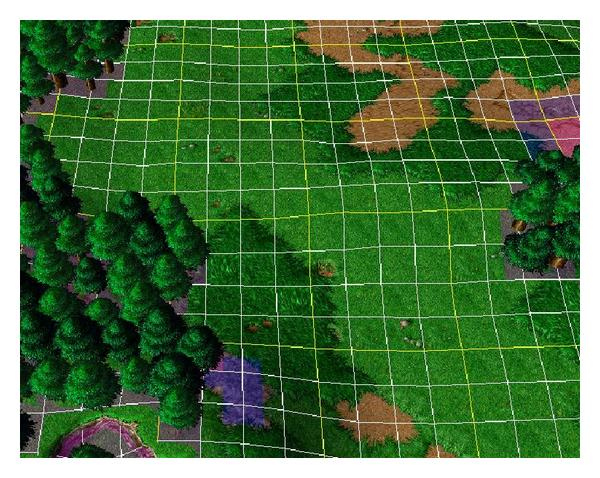
\includegraphics[width=0.5\columnwidth]{img/games/warcraft-map-editor}
	\caption{Ciągła przestrzeń mapy zdyskretyzowana do siatki pól. \\ Źródło: edytor map z gry Warcraft III.}
	\label{fig:img_games_warcraft-map-editor}
\end{figure}

Popularne podejścia unikające planowania w wysoko wymiarowej zbiorowej przestrzeni konfiguracyjnej to techniki rozproszone i uwzględniające priorytety \cite{optpriorities}.
Pomimo, że metody te są bardzo efektywne, mają dwie główne wady:
\vspace{-0.5em}
\begin{itemize}[itemsep=0em]
	\item Nie są zupełne - nie dają gwarancji znalezienia rozwiązania, nawet gdy takie istnieje.
	\item Wynikowe rozwiązania mogą być nieoptymalne.
\end{itemize}

% TODO-MGR
% W artykule \cite{optpriorities} przedstawione zostało podejście do optymalizowania układu priorytetów dla rozproszonych i uwzględniających priorytety technik planowania.
% Proponowana metoda wykonuje randomizowane przeszukiwanie z techniką hill-climbing do znalezienia rozwiązania i do skrócenia całkowitej długości ścieżek.
% Technika ta została zaimplemenotwana i przetestowana na prawdziwych robotach oraz w rozległych testach symulacyjnych, dając zadowalające rezultaty.

\section{Planowanie uwzględniające priorytety}
Często używaną w praktyce metodą jest planowanie z uwzględnianiem priorytetów. 
W tej technice agenci otrzymują unikalne priorytety. Algorytm wykonuje indywidualne planowanie sekwencyjnie dla każdego agenta w kolejności od najwyższego priorytetu. Trajektorie agentów o wyższych priorytetach są ograniczeniami (ruchomymi przeszkodami) dla pozostałych agentów \cite{async_decentralized_spacetime_cp}.

Złożoność ogólnego algorytmu rośnie liniowo wraz z liczbą agentów, dzięki temu to podejście ma zastosowanie w problemach z dużą liczbą agentów.
Algorytm ten jest zachłanny i niezupełny w takim znaczeniu, że agentów zadowala pierwsza znaleziona trajektoria niekolidująca z agentami wyższych priorytetów. 

Istotną rolę doboru priorytetów robotów w procesie planowania tras ukazuje prosty przykład przedstawiony na rysunku \ref{fig:image_article1_fig1}. Jeśli robot 1 (zmierzający z punktu S1 do G1) otrzyma wyższy priorytet niż robot 2 (zmierzający z S2 do G2), spowoduje to zablokowanie przejazdu dla robota 2 i w efekcie prawidłowe, istniejące rozwiązanie nie zostanie znalezione.
\begin{figure}
	\centering
	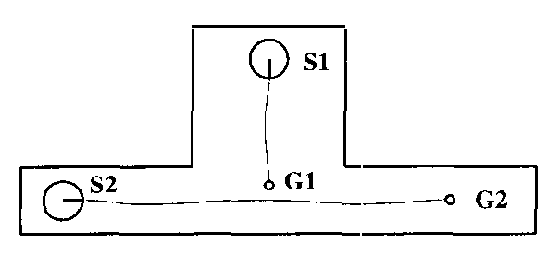
\includegraphics[width=6cm]{img/article1/fig1}
	\caption{Sytuacja, w której żadne rozwiązanie nie zostanie znalezione, stosując planowanie uwzględniające priorytety, jeśli robot 1 ma wyższy priorytet niż robot 2. Źródło: \cite{optpriorities}}
	\label{fig:image_article1_fig1}
\end{figure}

Układ priorytetów może mieć także wpływ na długość uzyskanych tras. Potwierdzający to przykład został przedstawiony na rysunku \ref{fig:image_article1_ppt6}. W zależności od wyboru priorytetów, wpływających na kolejność planowania tras, otrzymujemy różne rozwiązania.
\begin{figure}
	\centering
	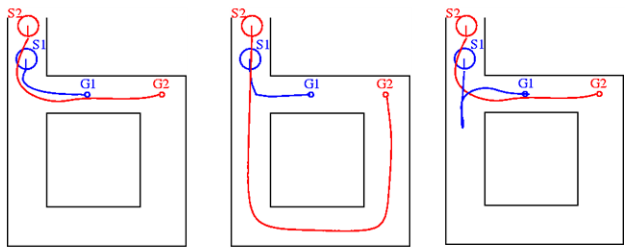
\includegraphics[width=13cm]{img/article1/ppt6}
	\caption{a) Niezależne planowanie optymalnych tras dla 2 robotów; b) suboptymalne rozwiązanie, gdy robot 1 ma wyższy priorytet; c) rozwiązanie, gdy robot 2 ma wyższy priorytet. Źródło: \cite{optpriorities}}
	\label{fig:image_article1_ppt6}
\end{figure}

\section{Metoda Path Coordination}
Jedną z metod rozproszonego planowania tras z uwzględnianiem priorytetów jest {\it Path Coordination}, której idea przedstawia się w następujących krokach \cite{optpriorities}:
\begin{enumerate}
	\item Wyznaczenie ścieżki dla każdego robota {\bf niezależnie} (np. za pomocą algorytmu A*)
	\item Przydział priorytetów
	\item Próba rozwiązania możliwych konfliktów między ścieżkami. Roboty utrzymywane są na ich indywidualnych ścieżkach (wyznaczonych na początku), wprowadzane modyfikacje pozwalają na zatrzymanie się, ruch naprzód, a nawet cofanie się, ale tylko {\bf wzdłuż trajektorii} w celu uniknięcia kolizji z robotem o wyższym priorytecie.
\end{enumerate}

\section{Wyznaczanie trajektorii dla pojedynczego robota}
\label{ch:alg-single-astar}

Wiele technik planowania tras, mimo iż może posłużyć do koordynacji ruchu wielu robotów, korzysta z metod indywidualnego planowania dla każdego agenta z osobna. Przykładem takiego podejścia jest {\it Local-Repair A*}, w którym to głównym algorytmem przeszukującym jest A*.
Z tego powodu przed przystąpieniem do opracowania bardziej skomplikowanych metod, należy najpierw zająć się implementacją algorytmu poszukiwania najkrótszej drogi na dwuwymiarowej mapie z jednym robotem. Wymagane jest to nawet dla metody WHCA*, która pomimo, że operuje na węzłąch określonych w czasie i przestrzeni, to jednak w obliczaniu samej heurystyki wykorzystuje przestrzenny algorytm A*.
Ogólna zasada działania algorytmu A* wraz z kluczowymi pojęciami została opisana w rozdziale \ref{ch:astar-theory}.

Pseudoko \ref{alg:astar} oraz opisy użytych pomocniczych funkcji ukazują szczegóły implementacji metody wyznaczania najkrótszej drogi na przestrzennej mapie. Algorytm oparty jest o A*, jednak posiada własne, niewielkie modyfikacje.

\begin{algorithm}[H]
	\caption{Algorytm A*}\label{alg:astar}
  \begin{algorithmic}[1]
\Function{znajdzDrogę}{$mapa$, $start$, $cel$}
	\State $closed \gets \varnothing$  \Comment{pusta lista zamkniętych}
	\State $open \gets \{start\}$ \Comment{lista otwartych zawiera punkt startowy}

	\For{$wezel \in mapa$}
		\State $wezel.g = \infty$ \Comment{domyślnie nieskończony koszt - odległość od startu}
	\EndFor

	\State $start.g \gets 0$ \Comment{Zerowy koszt przejścia do węzła startowego}

	\While{$open \ne \varnothing$} \Comment{dopóki lista otwartych nie jest pusta}
		\State $obecny \gets $ \Call{znajdźMinF}{$open$} \Comment{Szukamy pola o najniższej wartości f}

		\If{$obecny == cel$}
			\State \Return \Call{zbudujŚcieżkę}{$cel$} \Comment{Znaleziono ścieżkę}
		\EndIf

		\State dodaj $obecny$ do $closed$ \Comment{Przesunięcie z $open$ do $closed$}
		\State usuń $obecny$ z $open$
		
		\For{$sasiad \in$ \Call{sąsiedzi}{$obecny$}} \Comment{Dla każdego sąsiada aktualnego pola}
			
			\If{$mapa[sasiad.x][sasiad.y] == ZABLOKOWANE$ {\bf or} 
				\State {\bf not} \Call{przejściePoprawne}{$obecny$, $sasiad$}}
				\State {\bf continue} \Comment{Ignoruj niepoprawne pola lub przejścia}
			\EndIf
			
			\State $nowyKoszt \gets obecny.g \ +$ \Call{kosztPrzejścia}{$obecny$, $sasiad$}

			\If{$nowyKoszt < sasiad.g$} \Comment{znaleziono korzystniejsze połączenie}
				\State usuń $sasiad$ z $open$ \Comment{konieczność ponownego przeliczenia}
				\State usuń $sasiad$ z $closed$ \Comment{jeśli $sasiad \in open$ lub $sasiad \in closed$}
			\EndIf

			\If{$sasiad \not\in open \land sasiad \not\in closed$}
				\State $sasiad.g \gets nowyKoszt$ \Comment{zapisanie nowego połączenia}
				\State $sasiad.h \gets$ \Call{heurystyka}{$sasiad$, $cel$}
				\State $sasiad.parent \gets obecny$ \Comment{pole $obecny$ rodzicem dla pola $sasiad$}
				\State dodaj $sasiad$ do $open$
			\EndIf

		\EndFor
	\EndWhile

	\State \Return $\varnothing$ \Comment{Przeanalizowano wszystkie węzły, brak istniejącej ścieżki}
\EndFunction
  \end{algorithmic}
\end{algorithm}

Wykorzystane zostały pomocnicze funkcje:
\begin{itemize}
	\item \textsc{znajdźMinF}($lista$) - Funkcja zwraca z listy pole o najniższej wartości $f$ (sumie kosztu i heurystyki);
	\item \textsc{zbudujŚcieżkę}($cel$) - Funkcja zwraca ścieżkę z punktu startowego do punktu $cel$ zbudowaną na podstawie przechodzenia wstecz od punktu $cel$ po kolejnych rodzicach węzłów, aż do dotarcia do węzła bez rodzica (punktu startowego).
	\item \textsc{sąsiedzi}($pole$) - Funkcja zwraca zbiór pól bezpośrednio sąsiadujących (dla których istnieje możliwość przejścia) ze wskazanym polem. Jest to zazwyczaj zbiór ośmiu sąsiadujących pól. Funkcja uwzględnia warunki brzegowe na granicach mapy.
	\item \textsc{przejściePoprawne}($poleZ$, $poleDo$) - Funkcja zwraca prawdę wtedy i tylko wtedy, gdy istnieje możliwość przejścia z $poleZ$ do $poleDo$. Gdy wykonywany jest ruch ukośny, ale na przynajmniej jednym polu sąsiadującym z $poleZ$ i $poleDo$ znajduje się przeszkoda, to taki ruch jest niepoprawny. Ruch ukośny agenta z punktu $(x_1, y_1)$ do $(x_2, y_2)$ możliwy jest tylko w przypadku, gdy na żadnym z czterech pól: $(x_1, y_1)$, $(x_2, y_1)$, $(x_1, y_2)$, $(x_2, y_2)$ nie znajduje się przeszkoda. W rzeczywistym środkowisku zabezpiecza to robota przed uderzaniem o wystający róg ściany.
	\item \textsc{kosztPrzejścia}($poleZ$, $poleDo$) - Funkcja zwraca koszt przejścia z $poleZ$ do $poleDo$. Jest to odległość w sensie metryki euklidesowej.
	\item \textsc{heurystyka}($poleZ$, $poleDo$) - Funkcja zwraca przewidywaną długość pozostałej drogi od $poleZ$ do $poleDo$. Jest to również odległość euklidesowa.
\end{itemize}

Potwierdzeniem poprawności zaimplementowania algorytmu wyznaczania najkrótszej ścieżki jest przykładowa droga przedstawiona na rysunku \ref{fig:robopath-astar-simple} pochodzącym z aplikacji. Warto zauważyć, że możliwy jest ruch ukośny robota, ale nie taki, który powodowałby kolizję z wystającym rogiem "ściany".

\begin{figure}
	\centering
	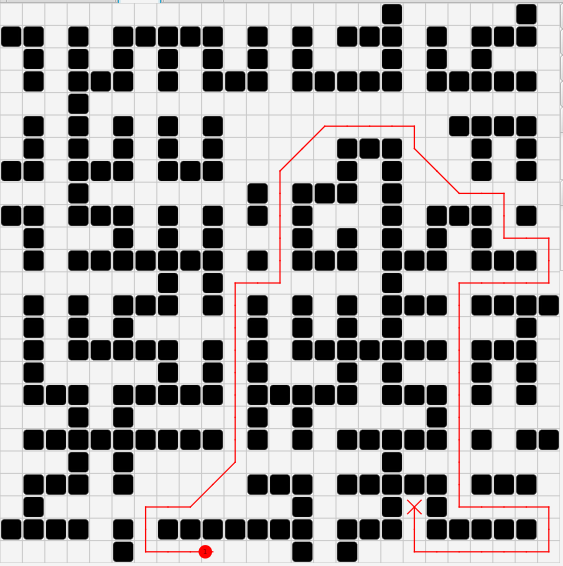
\includegraphics[width=0.7\columnwidth]{img/robopath/astar-simple}
	\caption{Przykładowa ścieżka wyznaczona przez zaimplementowany algorytm A*. Czarne kwadraty reprezentują przeszkody, kolorowe koło - robota, linia łamana - wyznaczoną ścieżkę.}
	\label{fig:robopath-astar-simple}
\end{figure}

% https://en.wikipedia.org/wiki/A*_search_algorithm

\section{Podsumowanie metod kooperacyjnego planowania}

Większość popularnych algorytmów wykorzystywanych do planowania tras dla wielu robotów mobilnych (agentów) opiera się o A*.

Kooperacyjne planowanie tras jest ogólną techniką koordynacji dróg wielu jednostek.
Znajduje zastosowanie, gdzie wiele jednostek może komunikować się ze sobą, przekazując informację o ich ścieżkach.
Poprzez planowanie wprzód w czasie, jak również i w przestrzeni, jednostki potrafią schodzić sobie z drogi nawzajem w celu uniknięcia kolizji.
Metody kooperacyjnego planowania są bardziej skuteczne i znajdują trasy wyższej jakości niż te uzyskane przez A* z metodą {\it Local Repair}.

Wiele z udoskonaleń przestrzennego algorytmu A* może być również zaadaptowane do czasoprzestrzennego A*.
Ponadto, wprowadzenie wymiaru czasu otwiera nowe możliwości do rozwoju algorytmów znajdowania dróg.

Najbardziej obiecującym pod względem skuteczności algorytmem wydaje się być metoda WHCA*.

Aby wydajnie prowadzić obliczenia, zakłada się, że każdy ruch robota trwa tyle samo. 
Wprowadza to upraszczające, błędne założenie, że ruch robota na pole w kierunku poziomym lub pionowym trwa tyle samo, co na ukos.

W wielu przypadkach metody do planowania bezkolizyjnych tras w systemach wieloagentowych mogą być wykorzystywane zamiennie zarówno do wyznaczania trajektorii robotów mobilnych, jak i w grach komputerowych, np. strategiach czasu rzeczywistego do planowania tras wielu jednostek.

Zaprezentowane algorytmy mogą znaleźć zastosowanie również w środowiskach z ciągłą przestrzenią oraz w dynamicznych środowiskach, w których to ścieżki muszą być przeliczane po wykryciu zmiany na mapie.


\chapter{Opracowanie i implementacja algorytmów}
\label{ch:alg-impl}

Na potrzeby stworzenia oprogramowania symulacyjnego do planowania bezkolizyjnych tras dla wielu robotów mobilnych należało opracować i zaimplementować niezbędne algorytmy.

W tym rozdziale opisano algorytmy, które znalazły zastosowanie w stworzonej aplikacji służącej do symulacji ruchu robotów mobilnych. Należą do nich:
\begin{itemize}
	\item Generator labiryntów (por. \ref{ch:mazegen})
	\item Algorytm A* (por. \ref{ch:alg-single-astar})
	\item Algorytm LRA* (por. \ref{ch:alg-collision-avoid})
	\item Algorytm WHCA* (por. \ref{ch:alg-whca})
	\item Procedury obsługi dynamicznego przydzielania priorytetów oraz rozszerzania okna czasowego (por. \ref{ch:alg-priorities-allocation})
\end{itemize}

\section{Generator map}
\label{ch:mazegen}

W rozdziale \ref{ch:tests} opisano wyniki testów przeprowadzonych na losowo wygenerowanych środowiskach.
Do ich automatycznego utworzenia wykorzystano własny generator map, który zapewnia im pewne pożądane własności opisane poniżej.

Zastosowanie zwykłego losowania położenia przeszkód na mapie mogłoby spowodować, że do niektórych obszarów na mapie nie udałoby się znaleźć drogi, nawet mimo braku istnienia pozostałych agentów. Takie środowisko nie miałoby sensownego zastosowania w praktyce, w kooperacyjnym znajdowaniu tras.

Zależy nam, aby uzyskać środowisko cechujące się dużą liczbą przeszkód i wąskimi korytarzami, aby uwypuklić problem występowania wąskich gardeł. Jednocześnie chcemy, aby istniała możliwość przejścia między dwoma dowolnymi punktami na mapie.
Do rozwiązania problemu wygenerowania takich labiryntów posłużymy się teorią grafów i pojęciem grafu spójnego.

\begin{definition}{\bf Graf spójny\\}
	Graf spójny spełnia warunek, że dla każdej pary wierzchołków istnieje łącząca je ścieżka.
\end{definition}

Układ pól na mapie będziemy reprezentować jako graf.
W naszym przypadku wszystkie przejezdne pola na mapie są wierzchołkami grafu. Natomiast połączenia między sąsiednimi przejezdnymi polami (między którymi istnieje możliwość bezpośredniego przejścia) są krawędziami w grafie.

Aby zapewnić, że powstały graf będzie spójny, na początku losujemy jedno pole będące ziarnem rozrostu labiryntu, a następnie do takiego podgrafu dołączamy kolejne wierzchołki, łącząc je drogą na mapie. Krok ten powtarzamy do momentu, aż wszystkie wierzchołki zostaną dołączone.
W tym celu wykorzystamy dwie pomocnicze listy wierzchołków:
\begin{itemize}
	\item lista wierzchołków {\it odwiedzonych} - zawiera wierzchołki (pola) należące już do grafu tworzącego labirynt. Między wszystkimi wierzchołkami z listy {\it odwiedzonych} istnieje łącząca je droga - tworzą one graf spójny.
	\item lista wierzchołków {\it nieodwiedzonych} - zawiera nieodwiedzone wierzchołki (pola), które nie zostały jeszcze dołączone do labiryntu.
\end{itemize}

Kolejne kroki proponowanego algorytmu przedstawiają się następująco:
\begin{enumerate}
	\item Inicjalizacja pustych list wierzchołków: {\it odwiedzonych} i {\it nieodwiedzonych}.
	\item Zapełnienie całej mapy przeszkodami. Następnie, zaznaczenie co drugiego pola (wzdłuż każdego z wymiarów) jako wolne (por. rys. \ref{fig:etapy-generowania}a) i dodanie ich do listy {\it nieodwiedzonych}.
	\item Wylosowanie ziarna rozrostu labiryntu z listy {\it nieodwiedzonych}, przeniesienie go na listę {\it odwiedzonych}.
	\item Łączenie kolejnych wierzchołków nieodwiedzonych z wierzchołkami odwiedzonymi. Dopóki lista {\it nieodwiedzonych} nie jest pusta:
	\begin{enumerate}
		\item Wylosowanie wierzchołka z listy {\it nieodwiedzonych}.
		\item Znalezienie najbliższego dla niego (w sensie metryki miejskiej) sąsiada z listy {\it odwiedzonych}.
		\item Połączenie wierzchołków drogą poprzez "wyburzanie" przeszkód (zaznaczania pola jako wolne), przesuwając się w kierunku wierzchołka docelowego, najpierw wzdłuż osi poziomej, następnie wzdłuż osi pionowej (por. rys. \ref{fig:etapy-generowania}b).
	\end{enumerate}
\end{enumerate}

Pojedyncze dołączanie kolejnych wierzchołków do rozrastającego się grafu labiryntu zapewnia, że wynikowy graf również będzie grafem spójnym.

Algorytm \ref{alg:mazegen} przedstawia pseudokod, obrazujący szczegóły działania zaprojektowanej metody.

\begin{algorithm}
	\caption{Generowanie labiryntu}\label{alg:mazegen}
  \begin{algorithmic}[1]
\Function{generujLabirynt}{$w$, $h$} \Comment{$w$ - szerokość mapy, $h$ - wysokość mapy}
	\State $mapa[][] \gets$ nowa tablica $w \times h$ wypełniona wartościami $ZABLOKOWANE$

	\State $nieodwiedzone \gets \varnothing$, $odwiedzone \gets \varnothing$ \Comment{inicjalizacja pustych list}
	\For{$x \gets 0$; $x < w$; $x \gets x + 2$} \Comment{co drugi indeks szerokości}
		\For{$y \gets 0$; $y < h$; $y \gets y + 2$} \Comment{co drugi indeks wysokości}
			\State $mapa[x][y] \gets WOLNE$
			\State dodaj $mapa[x][y]$ do $nieodwiedzone$
		\EndFor
	\EndFor

	\State $ziarno$ $\gets$ losowe pole z $nieodwiedzone$
	\State dodaj $ziarno$ do $odwiedzone$ \Comment{przeniesienie do $odwiedzone$}
	\State usuń $ziarno$ z $nieodwiedzone$

	\While{$nieodwiedzone \ne \varnothing$} \Comment{dopóki $nieodwiedzone$ nie jest pusta}
		\State $nowePole$ $\gets$ losowe pole z $nieodwiedzone$
		\State $sasiad$ $\gets$ \Call{znajdźNajbliższegoSąsiada}{$odwiedzone$, $nowePole$}
		\State \Call{wyburzDrogę}{$mapa$, $nowePole$, $sasiad$}
		\State dodaj $nowePole$ do $odwiedzone$ \Comment{przeniesienie do $odwiedzone$}
		\State usuń $nowePole$ z $nieodwiedzone$
	\EndWhile

	\State {\bf return} $mapa[][]$
\EndFunction

\State 
\Function{wyburzDrogę}{$mapa$, $poleZ$, $poleDo$}
	\State $x \gets poleZ.x$
	\State $y \gets poleZ.y$
	\While{$x < poleDo.x$} \Comment{przesuwanie w prawo}
		\State $mapa[x\verb-++-][y] \gets WOLNE$ \Comment{zwiększenie $x$}
	\EndWhile
	\While{$x > poleDo.x$} \Comment{przesuwanie w lewo}
		\State $mapa[x\verb+--+][y] \gets WOLNE$ \Comment{zmniejszenie $x$}
	\EndWhile
	\While{$y < poleDo.y$} \Comment{przesuwanie w dół}
		\State $mapa[x][y\verb-++-] \gets WOLNE$ \Comment{zwiększenie $y$}
	\EndWhile
	\While{$y > poleDo.y$} \Comment{przesuwanie w górę}
		\State $mapa[x][y\verb+--+] \gets WOLNE$ \Comment{zmniejszenie $y$}
	\EndWhile
\EndFunction
  \end{algorithmic}
\end{algorithm}

Wyrażenie $x\verb-++-$ oraz $x\verb+--+$ oznacza odpowiednio postinkrementację oraz postdekrementację (dokonanie zwiększenia lub zmniejszenia o 1 {\bf po} wykorzystaniu wartości zmiennej w wyrażeniu).
Funkcja \textsc{znajdźNajbliższegoSąsiada} wyszukuje sąsiada dla pola $nowePole$ z listy $odwiedzone$. Wynik wyszukiwania jest najbliższy w sensie metryki miejskiej (metryki Manhattan).

Kolejne etapy generowania labiryntu zobrazowano na rysunku \ref{fig:etapy-generowania}.

\begin{figure}
    \centering
        \subfloat[]{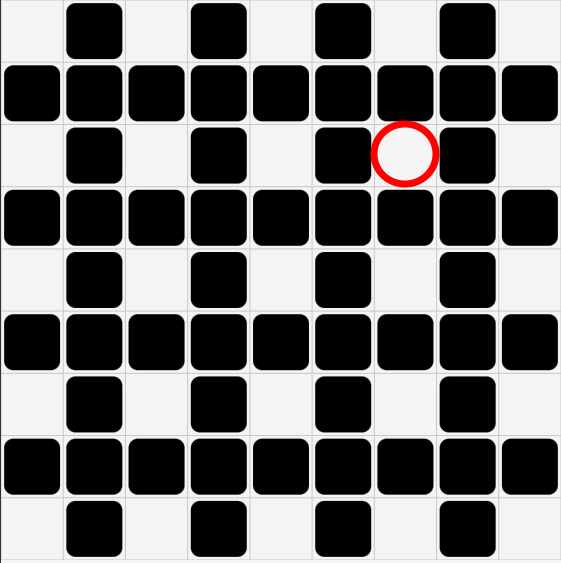
\includegraphics[width=0.3\columnwidth]{img/mazegen/maze-0initial-marks}}
        \qquad
        \subfloat[]{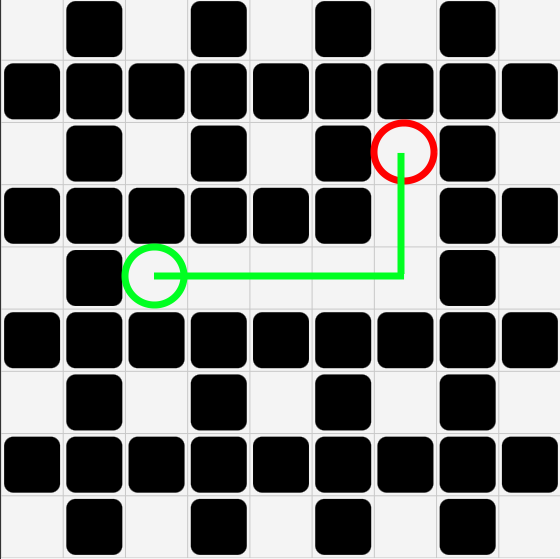
\includegraphics[width=0.3\columnwidth]{img/mazegen/maze-1cycle-marks}}
        \qquad
        \subfloat[]{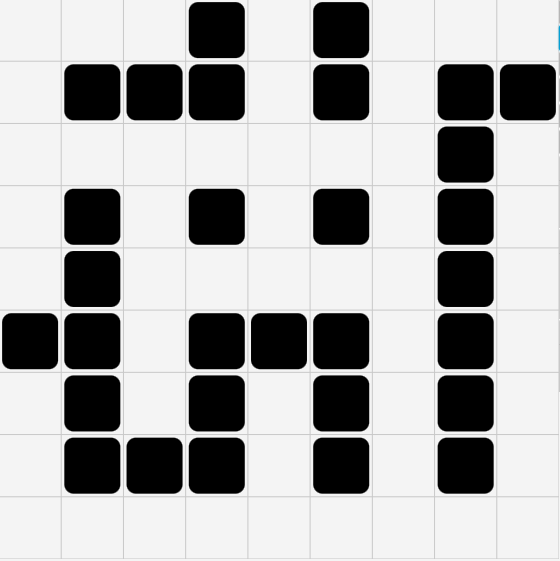
\includegraphics[width=0.3\columnwidth]{img/mazegen/maze-result}}
    \caption{Kolejne etapy generowania labiryntu:
    (a) Zaznaczenie co drugiego pola jako wolne i wybór ziarna rozrostu labiryntu.
    (b) Wylosowanie i łączenie kolejnego wierzchołka poprzez "wyburzanie" przeszkód na drodze
    (c) Wynikowa mapa pochodząca z generatora}
    \label{fig:etapy-generowania}
\end{figure}

Na rysunku \ref{fig:maze75-75} przedstawiono przykładowy labirynt wygenerowany opisanym algorytmem.
\begin{figure}
	\centering
	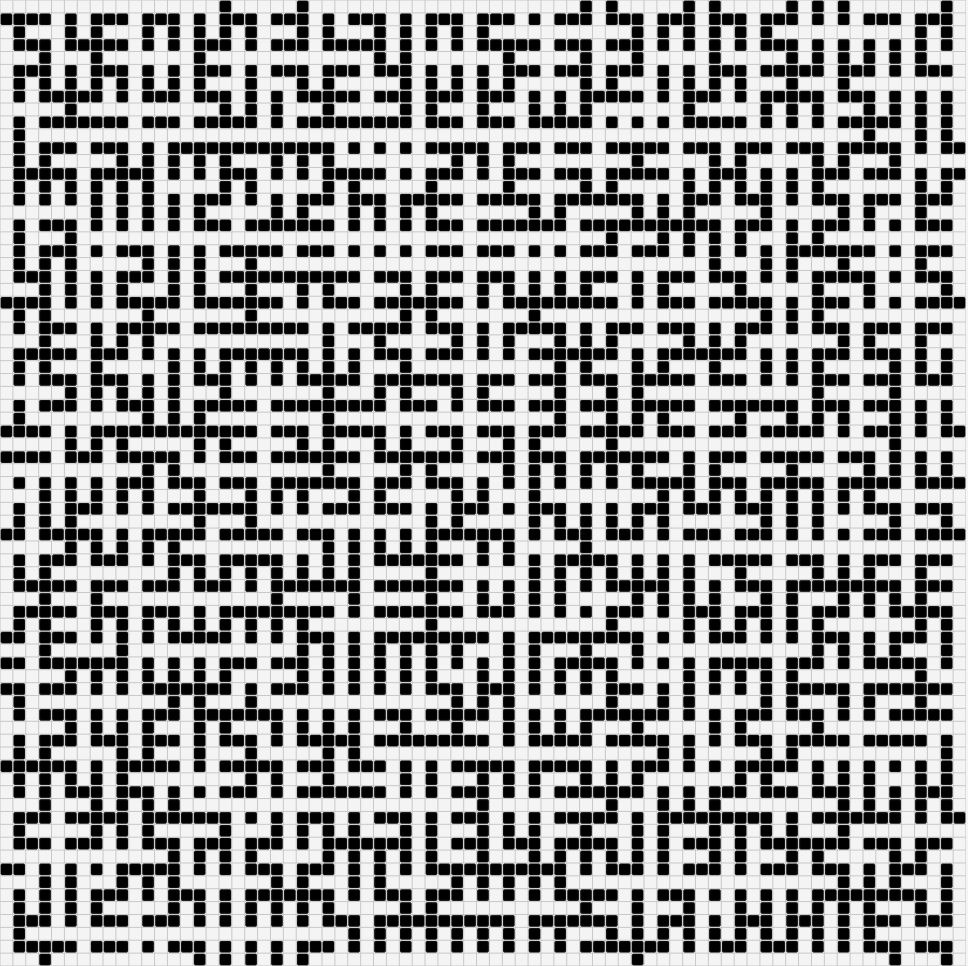
\includegraphics[width=0.6\columnwidth]{img/mazegen/maze-75-75}
	\caption{Przykładowy labirynt rozmiaru $75 \times 75$ pochodzący z zaprojektowanego generatora map}
	\label{fig:maze75-75}
\end{figure}

Warto zaznaczyć, że łączenie kolejnych wierzchołków do najbliższego sąsiada nadaje pewną właściwość wygenerowanym mapom.
Bardzo często (choć nie zawsze) między dwoma polami tworzy się tylko jedna łącząca je ścieżka (nie ma alternatywnych ścieżek). Sprzyja to tworzeniu się wąskich gardeł na mapie.

Wygenerowane w ten sposób mapy mają jeszcze jedną właściwość - w takim środowisku robot nie ma nigdy możliwości wykonania ruchu ukośnego (innego niż w poziomie lub pionie). Pozwoliłoby to wprowadzić pewne ograniczenia do niektórych algorytmów planowania (por. \ref{ch:theory-coop-astar}), które to przyspieszyłyby wykonywanie obliczeń ze względu na możliwość założenia jednakowego czasu trwania wszystkich ruchów robotów. Nie będziemy jednak tego zakładać na tym etapie, gdyż chcemy, aby opracowana metoda planowania tras mogła także działać w środowiskach o innym charakterze.


\section{LRA*}
$TODO$ wyszło całkiem nieźle, raczej nie potrzeba przydziału priorytetów, można łączyć z D* Lite lub D* Extra Lite, lub RRA
\section{Algorytm WHCA*}
\label{ch:alg-whca}

$TODO$ rozwiązuje bottleneck ale tylko dla małej liczby agentów (2)

WHCA2 - własny, schemat blokowy, pseudokod
\section{Dynamiczny przydział priorytetów}
\label{ch:alg-priorities-allocation}
Obok samego algorytmu WHCA* zrealizowano własną metodę dynamicznego przydziału priorytetów oraz skalowania okna czasowego, która to przyczynia się do zwiększenia skuteczności planowania ruchu robotów. Stanowi ona niejako rozwinięcie metody WHCA* o dodatkowe procedury.
Dla rozróżnienia poszczególnych wariantów metody WHCA* w dalszej części pracy będziemy posługiwać się skrótowymi nazwami:
\begin{itemize}
	\item {\bf WHCA*1} - {\it Windowed Hierarchical Cooperative A*} bez dynamicznego przydzielania priorytetów, ze stałym oknem czasowym,
	\item {\bf WHCA*2} - {\it Windowed Hierarchical Cooperative A*} z dynamicznym przydziałem priorytetów, ze stałym oknem czasowym,
	\item {\bf WHCA*3} - {\it Windowed Hierarchical Cooperative A*} z dynamicznym przydziałem priorytetów oraz skalowaniem okna czasowego.
\end{itemize}

Układ priorytetów w metodzie WHCA* ma istotny wpływ na wynik planowania tras.
Priorytety robotów warunkują kolejność wyznaczania ich dróg.
Z tego powodu robot o wyższym priorytecie podczas planowania nie będzie uwzględniał agentów o priorytetach niższych, gdyż planowanie ich dróg odbywa się później.
Może to zatem spowodować wyznaczenie trasy kolizyjnej z robotem o niższym priorytecie.

\subsection{Detekcja kolizji}
Podobnie jak w algorytmie LRA*, również w metodzie WHCA* należy wykrywać kolizje (odpowiednio wcześniej).
Nawet w przypadku, gdy roboty podążają wzdłuż zaplanowanych ścieżek, wciąż istnieje możliwość wystąpienia kolizji.
Taka sytuacja może wystąpić, gdy robot, który planuje drogę wcześniej (ma wyższy priorytet), nie uwzględnia, że następnemu robotowi może nie udać się wyznaczenie trajektorii (z powodu właśnie zaplanowanej trasy).
Wykrywanie kolizji odbywa się tak samo, jak w przypadku metody LRA* (por. \ref{ch:alg-collision-avoid}).
Należy zaznaczyć, że pod pojęciem wykrywania kolizji rozumiemy wczesne zauważenie kolizji, która wystąpiłaby w następnym kroku. Niepożądane jest doprowadzanie do faktycznych kolizji, dlatego interwencja zachodzi odpowiednio wcześniej.

% TODO screen z przypadku kolizjii

\subsection{Wariant WHCA*2}
%TODO stała wartość okna
Wariant WHCA*2 został wzbogacony o dynamiczny przydział priorytetów agentów.
Zaproponowane podejście polega na zwiększaniu priorytetów robotów w przypadku niepowodzenia w znalezieniu trasy.
Opiera się to na następujących krokach:
\begin{enumerate}
	\item Początkowo roboty mają nadane priorytety losowo. Otrzymują kolejne wartości od 1 do liczby wszystkich robotów.
	\item Rozmiar okna czasowego jest zawsze równy całkowitej liczbie agentów zwiększonej o 1.
	\item Planowanie tras dla robotów wykonywane jest w przypadku detekcji kolizji w poprzednim kroku symulacji, lub gdy robot wykonał już wszystkie akcje z jego indywidualnej kolejki akcji.
	Lista robotów zostaje posortowana malejąco według priorytetów przed wykonaniem planowania tras. Wyższa wartość priorytetu oznacza pierwszeństwo podczas planowania.
	\item Następnie wykonywane jest planowanie tras zgodnie z aktualnym układem kolejności robotów (jak w wariancie WHCA*1). Wyznaczone ścieżki zaznaczane są kolejno w tablicy rezerwacji.
	\item Jeśli dla któregoś robota nie została znaleziona bezkolizyjna ścieżka, to następuje zwiększenie jego priorytetu o wartość 1. Taki awans priorytetów może nastąpić dla wielu robotów w jednym kroku symulacji.
	\item Dla wszystkich robotów dokonywana jest weryfikacja wystąpienia kolizji. W przypadku jej wykrycia, kolejka ruchów obydwu (lub więcej) robotów zostaje opróżniona.
	\item W następnych krokach symulacji zostanie podjęta próba ponownego poszukiwania tras dla robotów, u których wystąpiło niepowodzenie planowania lub została wykryta kolizja. Tym razem nastąpi to z nowym układem priorytetów.
\end{enumerate}

Algorytm przewiduje możliwość posiadania przez wiele robotów tych samych wartości priorytetów.
Kolejność planowania dla takich robotów zależy wtedy od zastosowanego algorytmu sortowania list. W obecnej implementacji kolejność ta pozostaje taka sama, jak sprzed wystąpienia awansu priorytetów.

Warto dodać, że w sytuacji przedstawionej na rysunku \ref{fig:whca-giveway} metoda WHCA*2 byłaby w stanie doprowadzić roboty do celu niezależnie od początkowego układu priorytetów.

W przypadku wykrycia kolizji wielu robotów zwiększenie priorytetu dokonywane jest dla robota o niższym priorytecie.
Może to jednak prowadzić do naprzemiennego zwiększania priorytetów robotów powtarzającego się w nieskończonym cyklu.
Taki przypadek ilustruje rysunek \ref{fig:whca2-head}.
Robot nr 2 (niebieski) posiada priorytet równy 2 i wyznacza trasę jako pierwszy. Nie uwzględnia on robota nr 1 (czerwonego), dlatego wyznacza drogę po linii prostej do swojego celu, która koliduje z robotem nr 1.
W wyniku wykrytej kolizji zwiększa się priorytet robota nr 1 do wartości 3 (w dwóch kolejnych krokach symulacji) i kolejność planowania tras robotów zostaje odwrócona.
Następnie zwiększany jest priorytet robota nr 2, co powoduje powstanie niekończącego się cyklu.
Okno czasowe jest zbyt małe, aby roboty uznały drogę "na około" jako korzystniejszą, gdyż wymaga to oddalenia się od celu.
\begin{figure}[H]
	\centering
		\subfloat[]{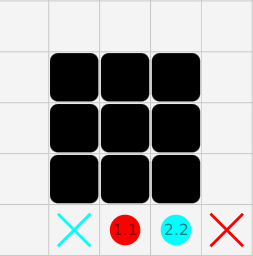
\includegraphics[width=0.3\columnwidth]{img/robopath/whca2-head-1}}
		\qquad
		\subfloat[]{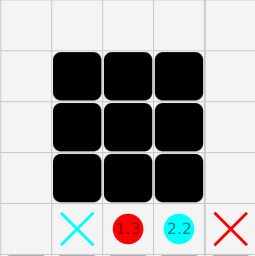
\includegraphics[width=0.3\columnwidth]{img/robopath/whca2-head-2}}
		\qquad
		\subfloat[]{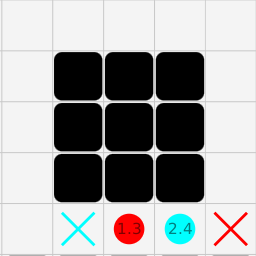
\includegraphics[width=0.3\columnwidth]{img/robopath/whca2-head-3}}
	\caption{Przykład cyklu naprzemiennego zwiększania priorytetów robotów uzyskanego metodą WHCA*2:
	(a) Robot nr 2 (niebieski) wyznacza trasę jako pierwszy, która koliduje z robotem nr 1 (czerownym).
	(b) Priorytet robota nr 1 zwiększa się do wartości 3.
	(c) Odwrócona kolejność planowania powoduje wzrost priorytetu robota nr 2.}
	\label{fig:whca2-head}
\end{figure}
Kolejny opisywany wariant WHCA*3 rozwiąże powyższy problem, wprowadzając w takich sytuacjach dodatkowe działanie.

\subsection{Wariant WHCA*3}
Wariant WHCA*3 stanowi rozszerzenie WHCA*2 o procedurę skalowania okna czasowego.
Rozmiar okna czasowego może zmieniać się w trakcie trwania symulacji.

Poniżej przedstawiono kroki wariantu WHCA*3. Modyfikacje w stosunku do wariantu WHCA*2 zostały w tekście wyróżnione (pogrubione). Wprowadzają one dodatkowe powiększanie okna czasowego do procedury dynamicznego przydziału priorytetów:
\begin{enumerate}
	\item Początkowo roboty mają nadane priorytety losowo. Otrzymują kolejne wartości od 1 do liczby wszystkich robotów.
	\item Rozmiar okna czasowego jest {\bf początkowo} równy całkowitej liczbie agentów zwiększonej o 1.
	\item Planowanie tras dla robotów wykonywane jest w przypadku detekcji kolizji w poprzednim kroku symulacji, lub gdy robot wykonał już wszystkie akcje z jego indywidualnej kolejki akcji.
	Lista robotów zostaje posortowana malejąco według priorytetów przed wykonaniem planowania tras. Wyższa wartość priorytetu oznacza pierwszeństwo podczas planowania.
	\item Następnie wykonywane jest planowanie tras zgodnie z aktualnym układem kolejności robotów (jak w wariancie WHCA*1). Wyznaczone ścieżki zaznaczane są kolejno w tablicy rezerwacji.
	\item Jeśli dla któregoś robota nie została znaleziona bezkolizyjna ścieżka, to następuje zwiększenie jego priorytetu o wartość 1. Taki awans priorytetów może nastąpić dla wielu robotów w jednym kroku symulacji.
	\begin{enumerate}
		\item {\bf Jeśli nowa wartość priorytetu robota przekracza aktualną wartość rozmiaru okna czasowego, to okno czasowe zostaje zwiększone do wartości równej maksymalnemu priorytetowi robota.}
	\end{enumerate}
	\item Dla wszystkich robotów dokonywana jest weryfikacja wystąpienia kolizji. W przypadku jej wykrycia, kolejka ruchów obydwu (lub więcej) robotów zostaje opróżniona.
	\item W następnych krokach symulacji zostanie podjęta próba ponownego poszukiwania tras dla robotów, u których wystąpiło niepowodzenie planowania lub została wykryta kolizja. Tym razem nastąpi to z nowym układem priorytetów.
\end{enumerate}

Rozszerzanie okna czasowego pozwala na poszukiwanie coraz bardziej skomplikowanych rozwiązań, gdy wciąż nie udaje się znaleźć rozwiązania. Jednocześnie nie przeznaczamy większej mocy obliczeniowej już na początku, gdy prawdopodobnie odbyłoby się planowanie w niepotrzebnie dużej głębi przeszukiwania.

Wariant WHCA*3 rozwiązuje w wielu przypadkach problem naprzemiennego, niekończącego się zwiększania priorytetów robotów.
Wraz ze wzrostem priorytetów zwiększa się okno czasowe i analizowane są bardziej skomplikowane rozwiązania.
Sytuację tą ilustruje rysunek \ref{fig:whca3-head}.
Warto zaznaczyć, że z tego typu problemem nie poradziła sobie metoda WHCA*2 (por. rys. \ref{fig:whca2-head}).
\begin{figure}[H]
	\centering
		\subfloat[]{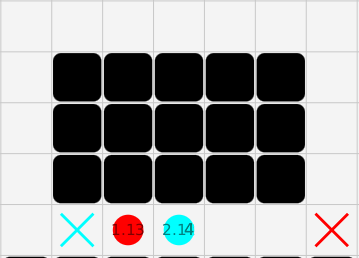
\includegraphics[width=0.3\columnwidth]{img/robopath/whca-head-4}}
		\qquad
		\subfloat[]{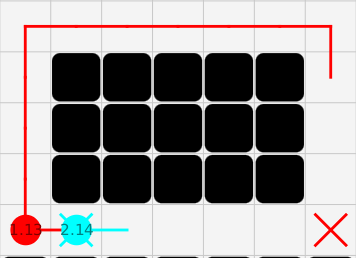
\includegraphics[width=0.3\columnwidth]{img/robopath/whca-head-5}}
		\qquad
		\subfloat[]{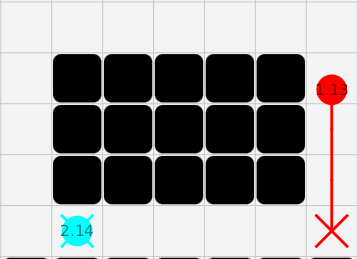
\includegraphics[width=0.3\columnwidth]{img/robopath/whca-head-6}}
	\caption{Przykład planowania tras metodą WHCA*3:
	(a) Priorytety robotów (oraz okno czasowe) wzrastają do wartości równej 14.
	(b) Wzrost rozmiaru okna czasowego powoduje odnalezienie alternatywnej drogi przez robota nr 1.
	(c) Po kolejnym planowaniu tras roboty osiągają punkty docelowe.}
	\label{fig:whca3-head}
\end{figure}

% TODO screeny ciekawych przypadków
% \begin{figure}
% 	\centering
% 	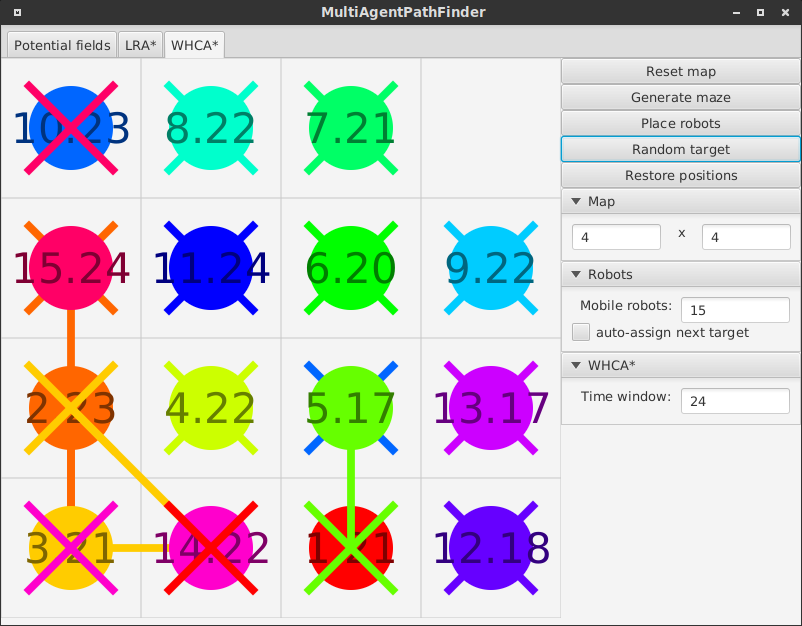
\includegraphics[width=0.8\columnwidth]{img/robopath/puzzle-15}
% 	\caption{Metoda WHCA*3: puzzle 15}
% 	\label{fig:test-puzzle-15}
% \end{figure}

Wykonane testy potwierdziły wzrost skuteczności w wyznaczaniu tras dzięki wprowadzeniu metody zarówno dynamicznego przydziału priorytetów jak i rozszerzania okna czasowego dla algorytmu WHCA* (por. \ref{ch:test-results}).

\chapter{Oprogramowanie symulacyjne}
\label{ch:simulation-app}

Na potrzeby pracy zostało stworzone oprogramowanie symulacyjne, które posłużyło do przeprowadzenia testów skuteczności algorytmów planowania tras oraz wizualizacji działania metod.
W tym rozdziale opisano techniczne rozwiązania wykorzystane podczas tworzenia oprogramowania.
W aplikacji zostały zaimplementowane algorytmy planowania tras opisane w rozdziale \ref{ch:alg-impl}.
Prezentacja ich działania odbywa się poprzez wizualizację ruchu robotów mobilnych w czasie rzeczywistym. 

\section{Funkcjonalności aplikacji}
Aplikacja umożliwia dowolne definiowanie przez użytkownika środowiska, w którym poruszają się roboty. Obejmuje to:
\begin{itemize}
	\item wybór rozmiaru mapy - dowolną wysokość oraz szerokość. Mapa nie musi być kwadratowa.
	\item możliwość wygenerowania mapy za pomocą generatora labiryntów (por. \ref{ch:mazegen}) lub manualnego umieszczania przeszkód na mapie za pomocą myszki,
	\item wybór liczby robotów i dokonanie ich automatycznego rozmieszczenia na mapie (w losowych polach z pominięciem pól zajętych). Użytkownik ma także możliwość manualnego dodawania i usuwania robotów.
\end{itemize}

Aplikacja przeprowadza symulację ruchu robotów w czasie rzeczywistym. W oprogramowaniu zostały zaimplementowane trzy algorytmy planowania ruchu robotów. Są to:
\begin{itemize}
	\item Metoda pól potencjałowych (por. \ref{ch:theory-potential-fields})
	\item Local-Repair A* (por. \ref{ch:alg-collision-avoid})
	\item WHCA*3 - Windowed Hierarchical Cooperative A* z dynamicznym przydziałem priorytetów oraz skalowaniem okna czasowego (por. \ref{ch:alg-whca}, \ref{ch:alg-priorities-allocation})
\end{itemize}
Wizualizacja każdego z tych algorytmów dostępna jest na osobnej zakładce w aplikacji.

\section{Metoda pól potencjałowych}
\label{ch:potential-fields}

W aplikacji zaimplementowano także metodę pól potencjałowych.
Cykl symulacji powtarzany jest w stałych cyklach zegarowych.
30 FPS
W każdym takim cyklu wyznaczana jest siła wypadkowa działająca na robota.
Wpływa to na zmianę wektora prędkości robota, a w konsekwencji na zmianę jego położenia.

Zastosowano działania na wektorach.

Siła "przyciągająca" robota do punktu docelowego ma stałą wartość, aby w każdej odległości od celu robot podążał do niego tak samo.

Wartość sumarycznej siły pochodzącej od wszystkich przeszkód jest ograniczana do maksymalnej wartości, aby wpływ od wielu przeszkód nie był na tyle znaczący, aby uniemożliwić robotowi dotarcie do celu.


zalety: real time - potrzeba mało obliczeń, szybka metoda

Problem minimów lokalnch
bardzo słaba skuteczność
siła z pięciu punktów przeszkody, a i tak efekt wallhacka
może się zderzyć z przeszkodą w wyniku nadmiernego rozpędzenia i braku wyhamowania, z powodu rozpatrywania jako punkty nie jako bryły

\chapter{Wyniki testów}
\label{ch:tests}

\section{Obszerne testy aplikacji}
$TODO$ obszerne testy, porównanie metod: LRA*, WHCA* przy tych samych warunkach początkowych, porównanie czasu wykonania, porównanie tego samego algorytmu w zależności od parametru (np. okna czasowego); badanie skuteczności, długości tras, czasu wykonania, 
do przeprowadzenia testów wykorzystano biblitekę jUnit, która co prawda służy do wykonywania testów jednostkowych sprawdzających poprawność pojedynczych komponentów aplikacji
metodyka przeprowadzenia testów
typy środowisk testowych (rozmiar, roboty, screeny):
	1. 11x11, 5 robotów
	2. 11x11, 10 robotów
	3. 35x35, 5 robotów
	4. 11x11 (bez labiryntu), 30 robotów
histogram liczby kroków potrzebnych do rozwiązania
potwierdzenie oczekiwań (poprawności) - nigdy nie było tak, żeby LRA był lepszy
zwykłego A* nawet nie warto testować
potential field - nawet nie warto testować, raczej jako ciekawostka, nie potrafi doprowadzić do celu nawet jednego robota
przeprowadzenie testów jest trudne i wymaga losowania środowisk i warunków i wyciągania statystyki

\section{Screeny}
$TODO$ screeny ciekawych przypadków

\begin{figure}
	\centering
	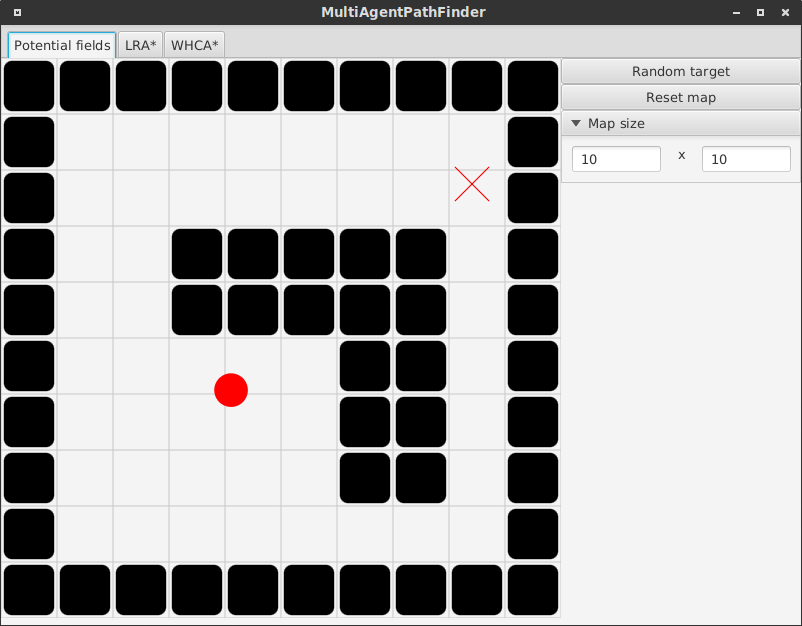
\includegraphics[width=0.8\columnwidth]{img/robopath/field-potential-hole}
	\caption{Robot uwięziony w studni potencjału. Zerowa siła wypadkowa nie pozwala mu dotrzeć do celu.}
	\label{fig:app-tech-intellij}
\end{figure}

\begin{figure}
	\centering
	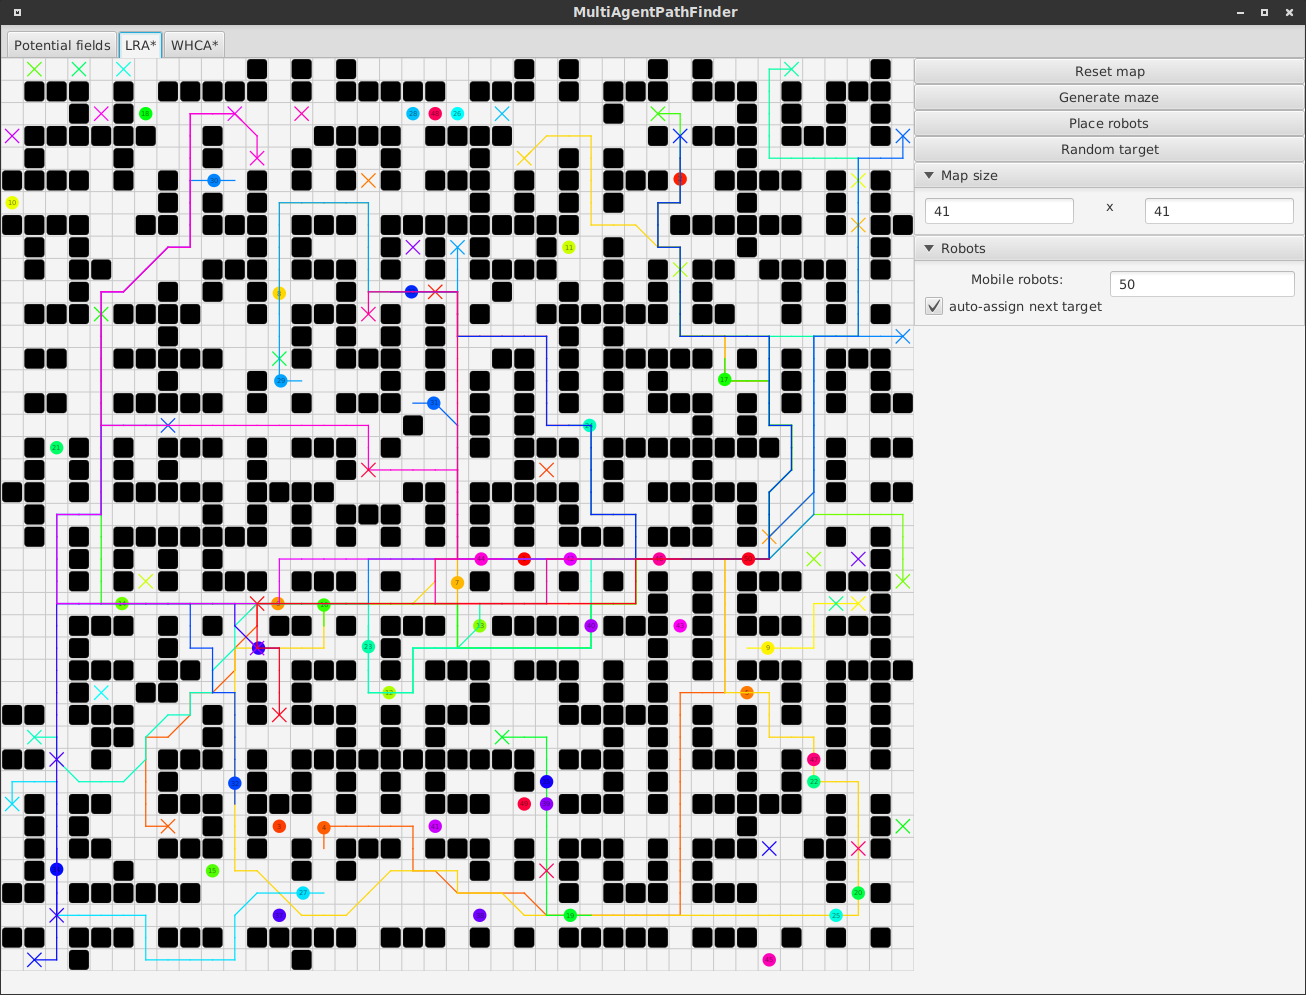
\includegraphics[width=0.8\columnwidth]{img/robopath/lra-bigmap}
	\caption{Metoda LRA*: duża mapa z dużą liczbą robotów}
	\label{fig:app-tech-intellij}
\end{figure}

\begin{figure}
	\centering
	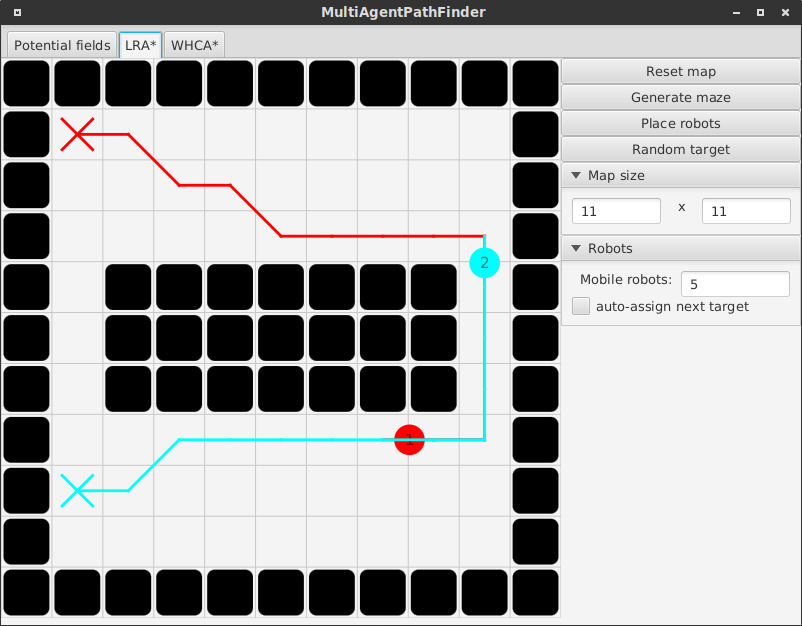
\includegraphics[width=0.8\columnwidth]{img/robopath/lra-cycle}
	\caption{Metoda LRA*: 2 roboty w cyklu akcji}
	\label{fig:app-tech-intellij}
\end{figure}

\begin{figure}
	\centering
	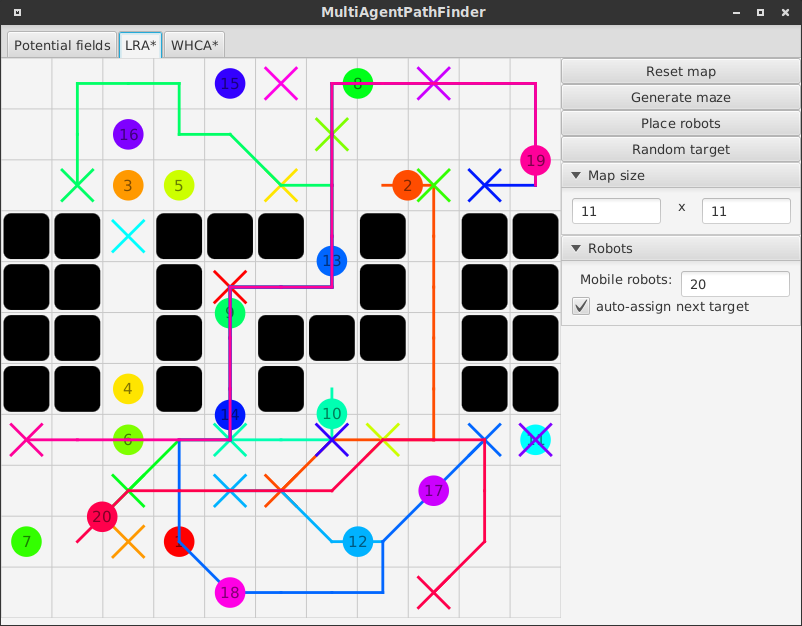
\includegraphics[width=0.8\columnwidth]{img/robopath/lra-lot-robots}
	\caption{Metoda LRA*: dużo robotów, mała mapa}
	\label{fig:app-tech-intellij}
\end{figure}

\begin{figure}
	\centering
	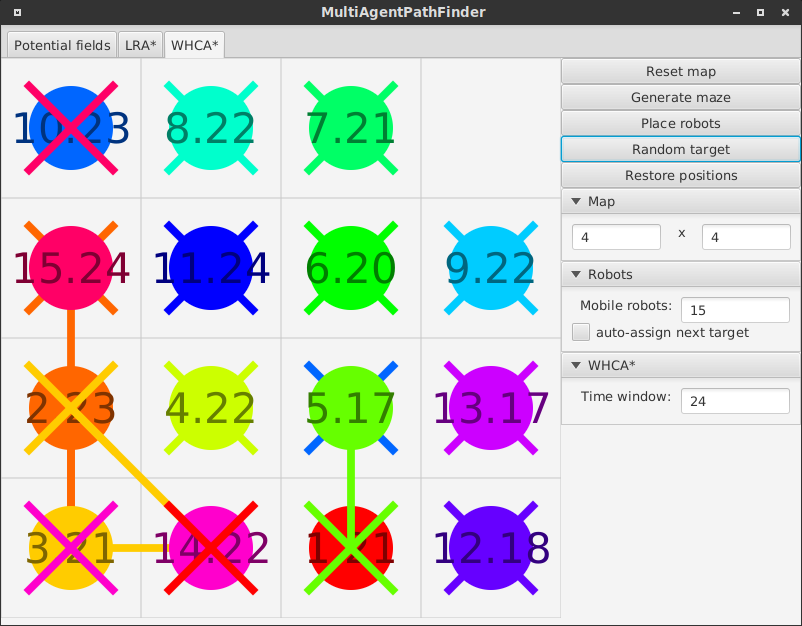
\includegraphics[width=0.8\columnwidth]{img/robopath/puzzle-15}
	\caption{Metoda WHCA*: puzzle 15}
	\label{fig:app-tech-intellij}
\end{figure}

\section{Środowiska}
labirynt, otwarte, puzzle 15

filmiki można obejrzć na YT, link

LRA: wyszło całkiem nieźle,
testy ograniczać trzeba liczbą kroków symulacji, bo LRA może trwać wiecznie

\section{Porównanie wyników}
jak często zwykły A* to za mało - ile razy pojawia się chociaż jedna kolizja?
porównanie WHCA* przy różnych oknach czasowych
porównanie metod przydziału i zmiany priorytetów - jak zmienia się skuteczność  po wprowadzeniu zmiany priorytetów
porównanie LRA* z WHCA*
porównanie CA* z WHCA*
porównanie z potential fields
porównanie WHCA z promocją priorytetów (własną, autorską) i bez + z/bez rozszerzania okna czasowego

\section{Dyskusja wyników}
wolno działa WHCA* przy dużych mapach / oknach czasu / robotach. Dałoby się zoptymalizować (RRA)
autorski WHCA* działa dobrze nawet przy rozwiązywaniu dużych deadlocków, problem z puzzle 15

wada - nie moze się dwóch agentów "cofać". MOże tylko uciekać  z drogi ważniesjzemu

\chapter{Podsumowanie}
\label{ch:podsumowanie}

$TODO$
Większość algorytmów Cooperative Pathfinding opiera się o A*

Algorytmy wprowadzają ograniczenie (błędne założenie), że ruchy trwają tyle samo. Można robić inaczej: podzielić dyskretnie i zaznaczać zajętość pól w wielu kratkach - ale wtedy będzie więcej obliczeń.

Windowed Hierarchical Cooperative A*:
• Cooperative A*
• Hierarchical Heuristic
• Windowed cooperation

The cooperative pathfinding methods are more successful
and find higher quality routes than A* with Local Repair.
Unfortunately, the basic CA* algorithm is costly to compute,

The size of the window has a significant effect on the suc-
cess and performance of the algorithm. With a large win-
dow, WHCA* behaves more like HCA* and the initialisa-
tion time increases. If the window is small, WHCA* be-
haves more like Local Repair A*. The success rate goes
down and the path length increases. The window size pa-
rameter thus provides a spectrum between Local Repair A*
and HCA*. An intermediate choice appears to give the most robust overall performance.
In general, the window size should be set to the duration
of the longest predicted bottleneck. In Real-Time Strategy
games groups of units are often moved together towards a
common destination. In this case the maximum bottleneck
time with cooperative pathfinding (ignoring units in other
groups) is the number of units in the group. If the window
size is lower than this threshold, bottleneck situations may
not be resolved well. If the window size is higher, then some
redundant search will be performed.

Local Repair A* may be an adequate solution for simple en-
vironments with few bottlenecks and few agents. With more
difficult environments, Local Repair A* is inadequate and is
significantly outperformed by Cooperative A* algorithms.

By introducing Hierarchical A* to improve the heuristic and
using windowing to shorten the search, a robust and efficient
algorithm, WHCA*, was developed. WHCA* finds more
successful routes than Local Repair A*, with shorter paths
and fewer cycles.

Although this research was restricted to grid environ-
ments, the algorithms presented here apply equally to more
general pathfinding domains. Any continuous environment
or navigational mesh can be used, so long as each agent’s
route can be planned by discrete motion elements. The grid-
based reservation table is generally applicable, but reserving
mesh intersections may be more appropriate in some cases.
Finally, the cooperative algorithms may be applied in dy-
namic environments, so long as an agent’s route is recom-
puted whenever invalidated by a change to the map.


Cooperative pathfinding is a general technique for coordinating the paths of many units.
It is appropriate whenever there are many units on the same side who are able to
communicate their paths. By planning ahead in time as well as space, units can get out of
each other’s way and avoid any conflicting routes.

Many of the usual enhancements to spatial A* can also be applied to space-time A*.
Moreover, the time dimension gives a whole new set of opportunities for pathfinding
algorithms to explore.


% \setpagenumberingtype{gobble} % Remove page numbers (and reset to 1)
\clearpage{\pagestyle{empty}\cleardoublepage}

% BIBLIOGRAFIA
\phantomsection
\addcontentsline{toc}{chapter}{Bibliografia}
\bibliographystyle{unsrt}	
\bibliography{bibliography}
\clearpage{\pagestyle{empty}\cleardoublepage}

% WYKAZ SKRÓTÓW
\phantomsection
\addcontentsline{toc}{chapter}{Wykaz skrótów}
\chapter*{Wykaz skrótów}

\begin{tabular}{l l}
API & Application Programming Interface \\
SDK & Software Development Kit \\


\end{tabular}

\clearpage{\pagestyle{empty}\cleardoublepage}

% SPIS RYSUNKÓW
\phantomsection
\addcontentsline{toc}{chapter}{Spis rysunków}
\listoffigures
\clearpage{\pagestyle{empty}\cleardoublepage}

% SPIS TABEL
\phantomsection
\addcontentsline{toc}{chapter}{Spis tabel}
\listoftables
\clearpage{\pagestyle{empty}\cleardoublepage}

% SPIS ZAŁĄCZNIKÓW
\phantomsection
\addcontentsline{toc}{chapter}{Spis załączników}
%\appendix
\chapter*{Spis załączników}

Na załączonej do pracy płycie CD znajdują się następujące treści:
\begin{itemize}
	\item Niniejsza praca w formacie PDF -- plik\\ \textit{Praca/Praca\_Magisterska\_Ireneusz\_Szulc.pdf}.

	\item Archiwum zawierające kody źródłowe programu symulacyjnego -- plik\\ \textit{Kody\_źródłowe/apliakcja-symulacja.zip}

\end{itemize}

% \clearpage{\pagestyle{empty}\cleardoublepage}

\end{document}
